\chapter{Úvod}
Při vývoji programů se často můžeme setkat s neuspokojujícími parametry jejich běhu -- ať už z hlediska času běhu nebo využití systémových zdrojů. Přes to, že cena hardware klesá a mzdy programátorů rostou, je často nutné přistoupit k optimalizaci existujícího kódu, namísto prostého přidání systémových prostředků \cite{mooreslaw}\cite{devsalary}. To sice v některých případech pomoci může, nicméně problém neřeší -- pouze jej oddaluje. Pokud chceme podobným problémům v budoucnu předejít a vyhnout se dalším investicím do výkonu, musíme problémový program upravit -- optimalizovat.

Optimalizace může probíhat na několika úrovních. První z možností může být volba efektivnějšího algoritmu -- můžeme zkontrolovat, zda jsme pro řešení problému zvolili vhodný algoritmus a zda neexistuje způsob, jakým bychom mohli dotyčné části řešit efektivněji. Tím je možné, především u vyššího počtu zpracovávaných prvků, dosáhnout výrazně rychlejšího běhu programu samotného. Dále je možné rychlost běhu ovlivnit zefektivněním (či prostou redukcí) přístupů k zařízením (IO), ať už se jedná o práci s diskem nebo síťovou činnost. Dále můžeme optimalizovat na úrovni využití systémových prostředků, typicky paměti (RAM). Právě optimalizaci paměťových nároků se v této práci budu věnovat.

I na snižování množství programem užité paměti lze pohlížet z několika různých úhlů. Navrhovaná řešení se mohou výrazně lišit dosaženými úsporami zdrojů, náročností či finanční nákladností. Jako první můžeme zvážit používané technologie. Změna programovacího jazyku je často natolik drahá, že kompletní přepsání dotyčného software ve většině případů nedává, i přes dosaženou optimalizaci, ekononomický smysl. V rámci námi používaného jazyku tak můžeme, kromě našeho kódu samotného, analyzovat používané frameworky a knihovny. V praxi se můžeme setkat s tím, že závislost na knihovně je přidána pouze z důvodu využití jedné či několika jejích funkcionalit. To je vhodné během vývoje z důvodu rychlosti; později je možné některé z těchto knihoven a jimi poskytované funkce nahradit implementací vlastní a teoreticky tak ušetřit jednotky, desítky či stovky megabytů paměti. Tím ovšem neoptimalizujeme data programu, ale velikost programu samotného.

Na řadu tak přichází právě programová data -- konkrétně datové struktury a typy, které v aplikaci jako její autoři využíváme. A opět je možné k tomuto problému přistoupit z různých úhlů, lišících se pak především hloubkou a důsledností analýzy. Můžeme řešit, zda námi používané typy odpovídají povaze dat -- například, zda rozsah celočíselného typu odpovídá maximální hodnotě dané veličiny.

V praxi mohou být následky nedůsledné optimalizace ještě vážnější. Systémy, které mají obsloužit vysoký počet požadavků za sekundu, je často nutné škálovat -- vytvářet nové, nezávislé jednotky těcho systémů. Ty se poté mohou střídat o příchozí požadavky. Každá neoptimalizace je tedy znásobena počtem těchto instancí. To může naprosto zbytečně zvyšovat náklady na provoz; a to ať už v případě vlastního serveru či cloudových služeb (tzv. serverless).

Cílem této práce je zanalyzovat, k jakým nedostatkům dochází (a zda vůbec) z pohledu neefektivního využití paměti při vývoji Java aplikací. Dále pak vytvořit nástroj, který na tyto nedostatky dokáže poukázat a uživateli napovědět, jakým způsobem by mohl použité prostředky svého programu redukovat a jeho běh tedy optimalizovat. Korektní fungování vytvořeného nástroje bude ověřeno na testovací aplikaci z pohledu správnosti a úplnosti výsledků. Následně pak také prověřeno na větších, rozšířených a běžně používaných Java aplikacích, za účelem posouzení efektivity použití nástroje v praxi, případně také v komerční sféře.



% =====================================================================================================================================================================================



\chapter{Problém správy paměti}
Při vytváření programu má jeho autor na výběr ze dvou způsobů správy paměti -- spravované automaticky (typicky mechanismem typu \zkratka{GC} apod.) či manuálně, případně kombinací těchto přístupů. Ne každý jazyk nabízí oba -- typicky je k dispozici pouze jeden z přístupů, často je správa GC vynucena. Vzhledem k tomu, že majorita nejpopulárnějších programovacích jazyků za poslední roky se řadí mezi vysokoúrovňové, na toto vynucení \zkratka{GC} narazíme u většiny z nich, včetně Javy \cite{stackoverflowinsights}\cite{tiobeindex}. Výjimkou jsou populární nízkoúrovňovější jazyky typu C a C++.

\section{Garbage collector}
\zkratka{GC} je nástroj, starající se o správu paměti programu -- její přidělování, kontrolu a následné uvolnění, ať už pokud je jí málo a je zapotřebí jinde, v pravidelných intervalech nebo při jiných událostech. \zkratka{GC} je obecný termín, tj. neodkazuje na žádnou konkrétní implementaci a způsob chování. Často je v rámci jednoho jazyka (respektive běhového prostředí) zároveň implementováno hned několik algoritmů \zkratka{GC} a dle okolností je vybrán ten nejefektivnější a v danou chvíli nejvhodnější z nich. Některé algoritmy tak mohou běžet velmi rychle bez minimálního zásahu do běhu programu, zatímco jiné vyžadují pro svůj běh o něco delší čas. Často tak je nutné všechen běh kódu pozastavit; v takových případech toto spuštění \zkratka{GC} nazýváme \textit{stop-the-world} (\uv{zastavení světa}, běhu). Pro program je toto zastavení transparentní.

Obecně \zkratka{GC} funguje tak, že si udržuje seznam referencí na jednotlivé objekty, respektive jejich počet. Pokud je některý z objektů dále nereferencovaný, při dalším běhu \zkratka{GC} bude jím zabíraná paměť uvolněna. Nereferencovaným objektem rozumíme, že je nedosažitelný -- nikdo na něj neukazuje. K takovým případům samozřejmě může docházet i v případě jazyků, které fungují bez \zkratka{GC}, např. \texttt{C}. Pokud daný jazyk nezná jiný způsob, jak se k dané paměti opětovně dostat, dochází k tzv. \textit{memory leakům}, tedy únikům paměti. V případě například výše zmíněného \texttt{C} nelze definitivně rozhodnout o nedostupnosti paměti -- díky ukazatelové aritmetice je možné paměť zpětně dopočítat i v případě, že v jednom časovém okamžiku na něj žádný ukazatel v paměti programu neukazuje. Java koncept ukazatelové aritmetiky nezná, po odstranění poslední reference si tedy můžeme být jisti, že už znovu referencovat nikdy nepůjde. V souvislosti s \textit{memory leaky} je nutné zdůraznit, že v tomto případě mám na mysli odstranění poslední reference v rámci paměti uživatelského programu. \zkratka{JVM}, který paměť spravuje, adresu objektu stále zná a je tak schopný jej v rámci běhu \zkratka{GC} odstranit.


% =====================================================================================================================================================================================

\chapter{Struktura paměti programu}

Abychom mohli hledat v paměti a analyzovat nedostatky v rámci jejího využití, musíme nejprve porozumět její struktuře, různým typům oblastí a objektům v nich uložených. Přestože se mnoho následujících konceptů a pravidel vztahuje na ostatní jazyky (a v některých případech i na paměť spravovanou samotným operačním systémem), budu se primárně zaměřovat Javu. Specifikace \zkratka{JVM} neobsahuje žádnou konkrétní podobu paměti či její rozložení, stejně tak jako nespecifikuje žádný konkrétní algoritmus \zkratka{GC} a žádné optimalizace, které se mají nad běžícím kódem vykonávat. Tyto implementační detaily jsou ponechány na možnostech a tvůrčích schopnostech vývojářů, kteří standard implementují. Prostým požadavkem tak je korektní načtení dat ze souboru \texttt{class} a validní vykonání příslušných instrukcí.

\zkratka{JVM}, stejně jako většina ostatních běhových prostředí a jazyků, rozeznává dva druhy datových typů -- primitivní a referenční. Proměnné primitivního typu tak obsahují přímo danou hodnotu, zatímco proměnné referenčních typů referencují (tj. ukazují na) jinde umístěnou paměť, v níž se nachází objekt.

Primitivních datových typů je v Javě několik druhů, konkrétně:

\begin{itemize}
	\item numerické
	\begin{itemize}
		\item celočíselné
			\begin{itemize}
				\item \texttt{byte}
				\item \texttt{short}
				\item \texttt{int}
				\item \texttt{long}
				\item \texttt{char}
			\end{itemize}
		\item s plovoucí desetinnou čárkou
			\begin{itemize}
				\item \texttt{float}
				\item \texttt{double}
			\end{itemize}
		\end{itemize}
	\item \texttt{boolean}
	\item \texttt{returnAddress}
		\begin{itemize}
			\item Speciální datový typ, sloužící jako pointer na \texttt{JVM} instrukce, konkrétně \texttt{jsr}, \texttt{ret} a \texttt{jsr\_w}. V běžném programu jej nicméně nemůžeme jako vývojáři použít ani modifikovat; \texttt{JVM} jej však zná a využívá.
		\end{itemize}
\end{itemize}

Referenční datové typy jsou potom následující:
\label{ref-types}
\begin{itemize}
	\item \texttt{class}
	\item \texttt{array}
	\item \texttt{interface}
\end{itemize}

Typ \texttt{array}, tedy pole, samozřejmě obsahuje seznam prvků určitého typu -- ten nazýváme typem komponenty. Proměnná referenčního typu je ukazatelem do paměti -- místa, kde je obsah objektu umístěn. Prázdný ukazatel, který nereferencuje žádné místo v paměti, nazýváme \texttt{null}. Tato hodnota je výchozí pro všechny proměnné referenčního typu, dokud jim není přiřazena hodnota \cite{jvms}. 

V násedujících odstavcích popisuji různé části paměti \texttt{JVM} -- viz obrázek \ref{obr-jvms-img}.

\section{JVM stack}
V případě, že v Javě mluvíme o stacku (zásobníku), typicky máme na mysli \zkratka{JVM} stack. Kromě něj totiž ještě existuje nativní stack, který je vytvořený operačním systémem pro potřeby \zkratka{JVM} samotného. Kromě toho je využívaný i pro některé nízkoúrovňovější činnosti. \zkratka{JVM} stack je spravovaný běhovým prostředím samotným a slouží pro potřeby aplikací, které v rámci prostředí běží.

Pro každé vlákno aplikace je vytvořený stack. Do něj jsou ukládány lokální proměnné, hodnoty parametrů metod a návratové hodmoty. Rovněž se stará o volání metod, respektive o návrat do volací metody po zavolání metody jiné. Stejně jako v jiných jazycích (třeba C) je paměť lokálních proměnných automaticky uvolněna při odebírání hodnot ze stacku. Takto alokovanou paměť tak není nutné spravovat \zkratka{GC} (či v případě C ručně uvolňovat).

Právě velikost \zkratka{JVM} stacku je často omezující faktor při vývoji, na který v některých případech (např. nesprávně zastavovaná rekurze) narážíme. Jeho velikost můžeme nastavit jako parametr při spuštění programu -- konkrétně \texttt{Xss} (respektive \texttt{-XX:ThreadStackSize}). Jeho výchozí velikost je závislá na velikosti dostupné (virtuální) paměti. V souvislosti s nedostatkem paměti a velikostí stacku se můžeme setkat se dvěma typy výjimek. \texttt{Stack\-Overflow\-Error} je vyhozena v případě, že během výpočtu narazíme na horní hranici velikosti stacku. \texttt{JVM} se případně může pokusit velikost dynamicky zvýšit. Pokud však během této operace narazí na velikost výše zmíněné paměti (což je už limitace nastavená operačním systémem a případně i hardwarovou konfigurací), je vyhozena výjimka jiná -- \texttt{OutOfMemoryError}. Tato výjimka je rovněž produkována v případě, že ručně nastavíme velikost stacku takovou, že při jeho vytváření \texttt{JVM} narazí na limity paměti rovnou.

\subsection{Rámce}
Rámce (\textit{frame}) přísluší právě jednomu stacku \ref{jvms-frames}. Data v něm jako takovém jsou totiž neměnná; jsou pouze přidávány/odebírány odkazy na rámce. V každém okamžiku je pro jedno vlákno aktivní právě jeden rámec. 

\subsubsection{Lokální proměnné}
Každý rámec obsahuje pole s lokálními proměnnými. Vzhledem k tomu, že je rámec vytvořen a vložen do \zkratka{JVM} stacku při volání metody a znovu odebrán a zničen při návratu z ní, právě toto pole zajišťuje uvolnení paměti alokovaných proměnných. Kromě promenných primitivního typu jsou v tomto poli uloženy rovněž reference na objekty v heapu (viz dále), jejich uvolnění sníží počet referencí na daný objekt a v případě dosažení nulové hodnoty je tento objekt připraven na uvolnění pomocí \zkratka{GC}.

\subsubsection{Stack operandů}
Tento stack slouží pro mezivýpočty při provádění operací, převážně matematických.

\section{Program counter registr}
\textit{Program counter} (PC) je registr s adresou ukazující na operaci, která se má provést. Vzhledem k tomu, že Java umožňuje vícevláknový běh, má samozřejmě každé vlákno svůj PC. 

\section{Stack nativních metod}
Pokud má daná implementace \zkratka{JVM} podporovat i tzv. \texttt{native} metody, měla by obsahovat i stack nativních metod. Zdůrazňuji, že \textit{měla} -- specifikace zde benevolentně ponechává rozhodnutí na konkrétním řešení a tento stack nutně nevynucuje. Díky konceptu nativních metod je možné přímo z Javy volat kód napsaný např. v C. 

Stejně jako \zkratka{JVM} stack, i stack nativních metod v některých případech produkuje výjimky. Toto chování je totožné pro oba stacky; stejně tak typy těchto chybových stavů jsou stejné.

\section{Heap}
Heap, tj. \textit{halda}, je část paměti, která je pro všechna vlákna programu společná a v Javě tomu není jinak. Díky tomu, že jsou všechny objekty alokovány právě v heapu, k nim můžeme přistupovat napříč metodami, objekty i vlákny. Platnost v ní umístěných objektů tak není omezena žádným blokem platnosti (snad jen s výjimkou běhu programu samotného) -- nedojde k uvolnění jimi zabírané paměti automaticky při opuštění tohoto bloku tak, jak je tomu v případě stacku. Právě kvůli tomu nad heapem operuje \zkratka{GC}, který nepotřebné objekty vyhledává a jejich paměť uvolňuje.

Kromě alokovaných objektů jsou rovněž v heapu uchovávány instanční proměnné. Právě z toho důvodu je nutné si dávat pozor na souběh při běhu ve více vláknech --  všechna při přístupu k instanční proměnní manipulují se stejným objektem.

I heap má samozřejmě omezenou velikost. Ta se dá nastavit dvěma přepínači:

\begin{itemize}
	\item \texttt{Xms} -- Výchozí velikost heap, s kterou Java nastartuje.
	\item \texttt{Xmx} -- Maximální velikost.
\end{itemize}

V případě 32 bitového systému jsou horní hranicí pro maximální velikost heapu 4 Gb, stejně jako v případě velikosti RAM (bez použití různých triků a rozšíření, jako třeba \textit{PAE}, apod.). Jak vyplývá z existence výše zmíněných přepínačů, \zkratka{JVM} dokáže s velikostí heapu dynamicky manipulovat. Program, respektive prostředí pro něj, tak spustí s výchozí hodnotou velikosti a v případě potřeby ji rozšiřuje (nebo naopak zmenšuje) až do maxima. Pokud si běh programu žádá více paměti v heapu, než může \zkratka{JVM} alokovat (tj. než má od systému k dispozici), vyhod, stejně jako v případě stacku, výjimku \texttt{OutOfMemoryError}. 

Heap je rozdělen dále do několika prostorů, jak je popsáno dále v kapitole \ref{memory-management}.

\section{Non-heap oblast}
Kromě oblasti metod bsahuje pomocná data, která jsou potřeba pro interní zpracování a potřeby. 
\subsection{Oblast metod}
Oblast, která uchováva data jednotlivých metod. Pro každou načtenou třídu uchovává strukturu se seznamem metod, statickými proměnnými a kódem metod a konstruktorů. Na jednu ze struktur třídy směřuje ukazatel z aktuálně zpracovávaného rámce v stacku, pomocí kterého může aktuálně vykonávaný kód přistupovat ke statickým členům třídy.

\begin{figure}[h]
	\centering
	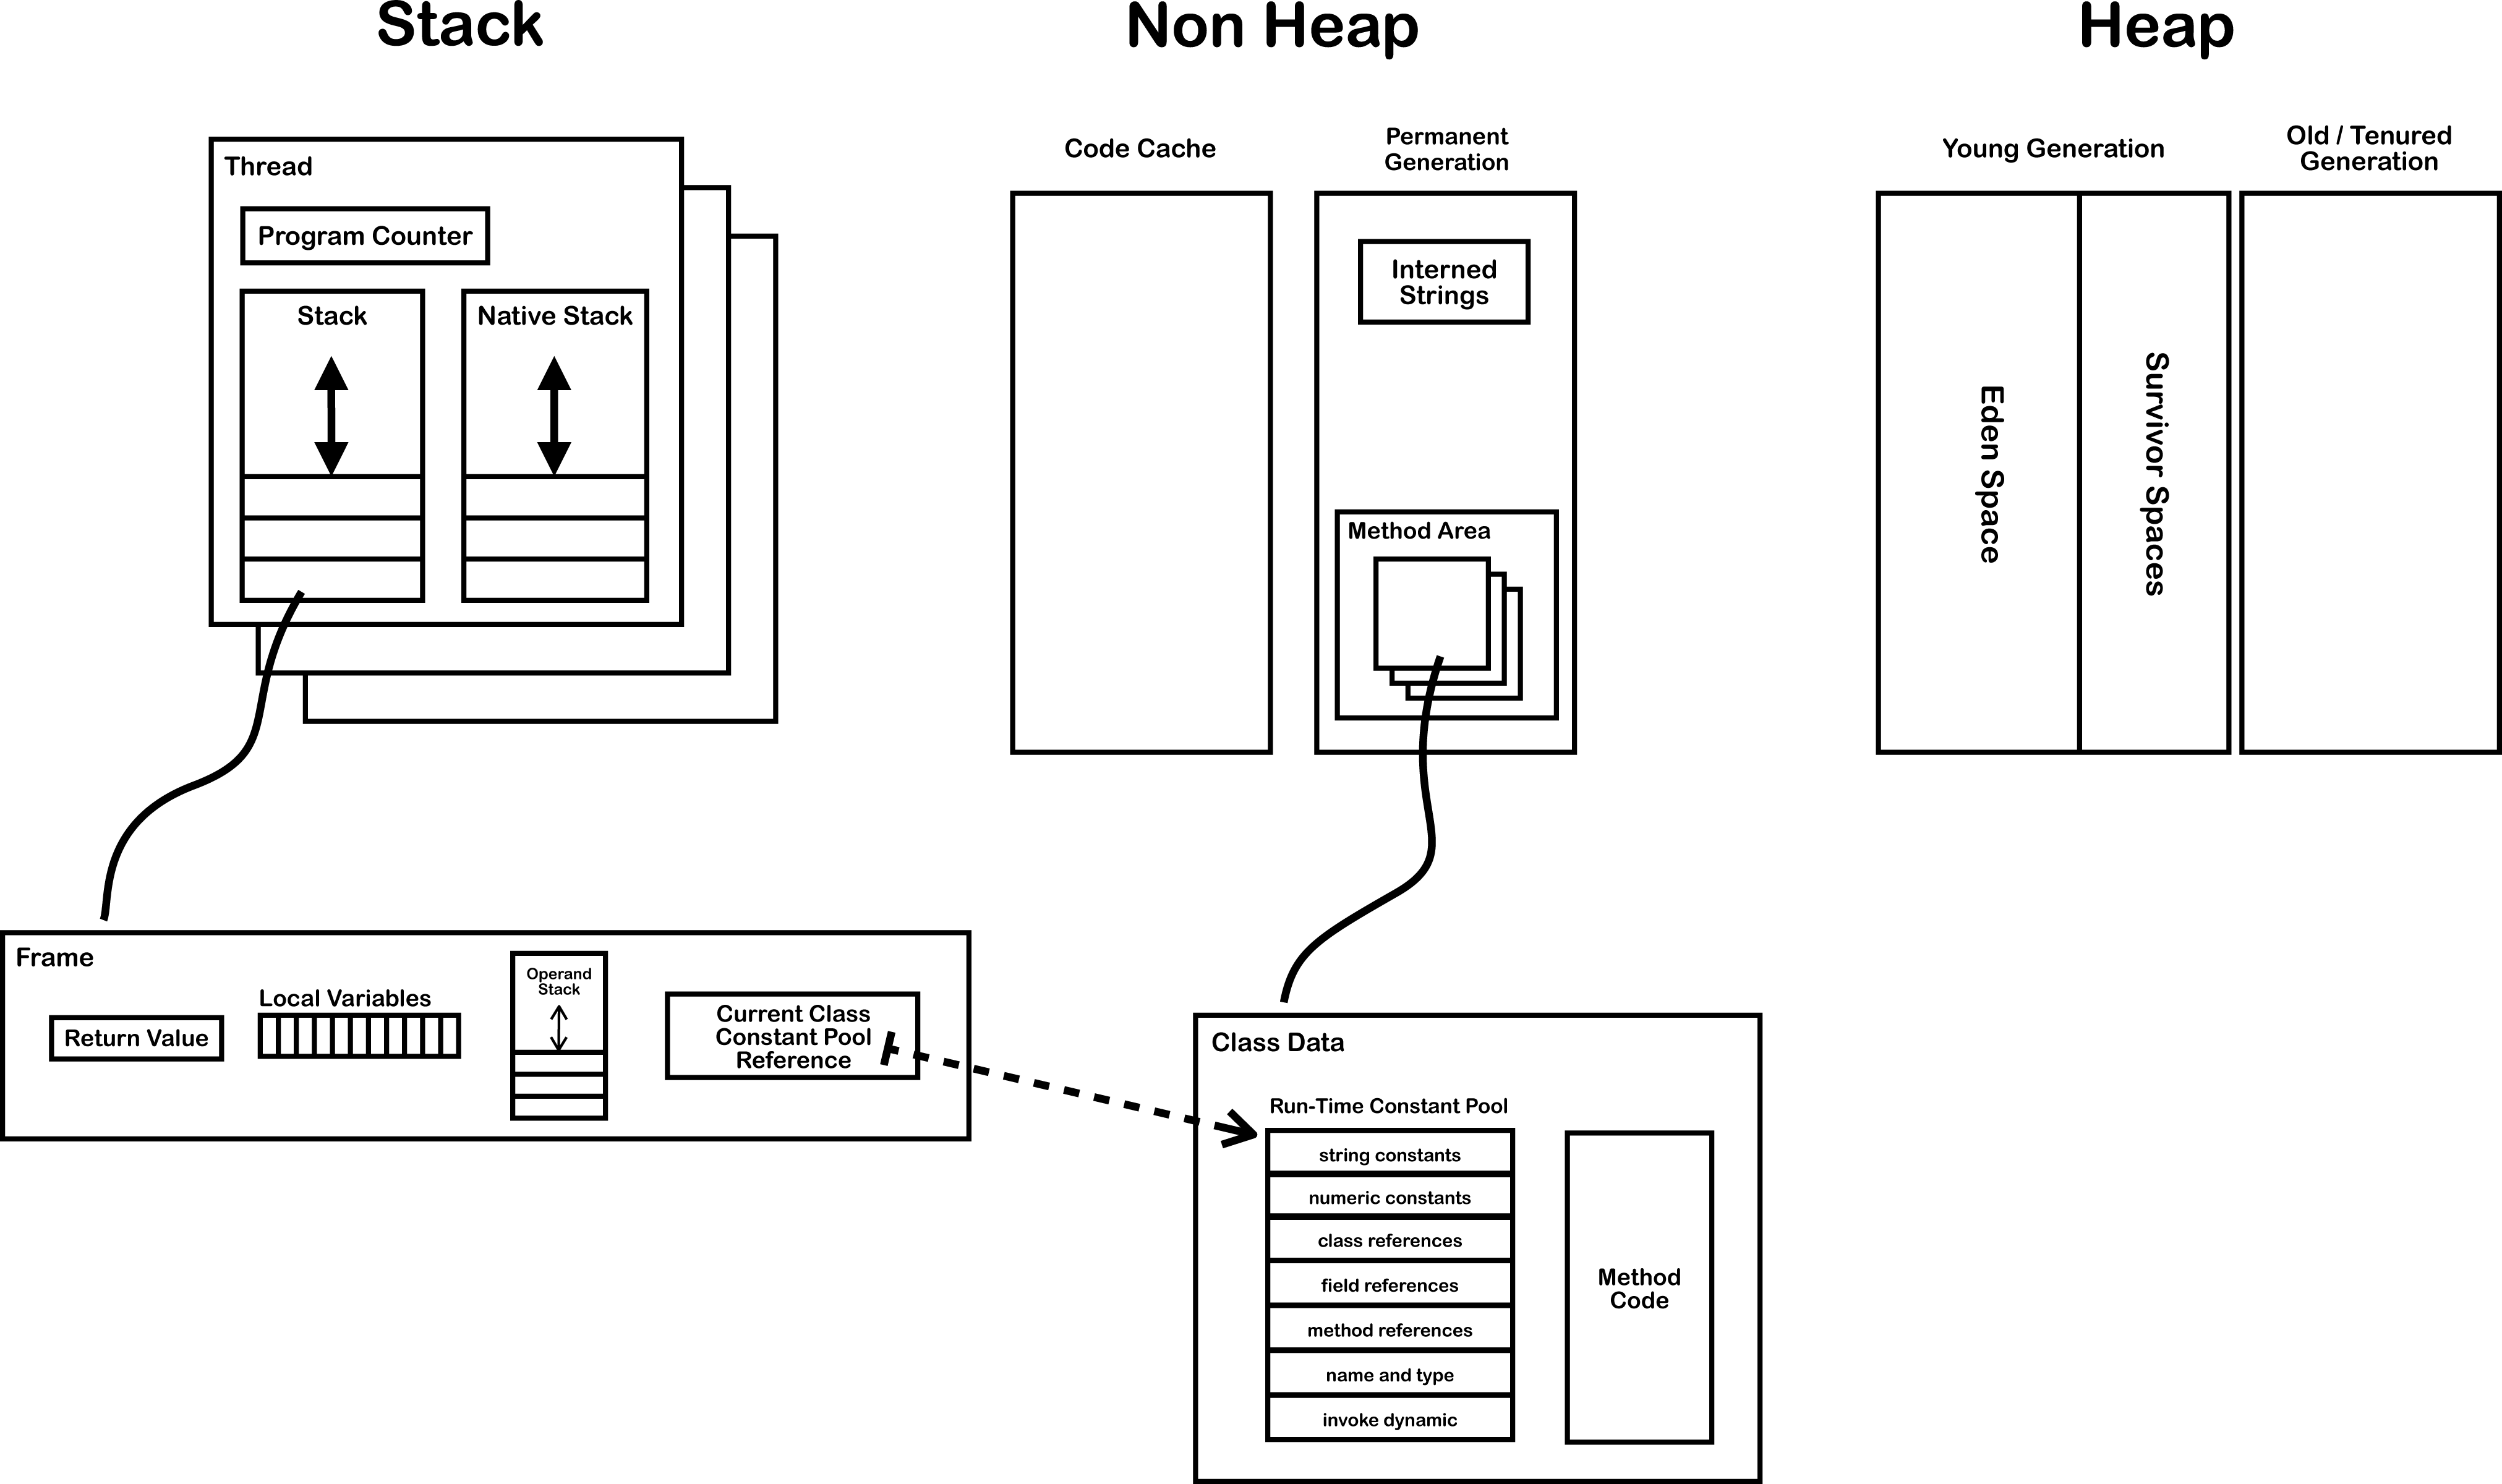
\includegraphics[scale=0.1]{obrazky/JVM_Internal_Architecture.png}
	\caption{Struktura Java paměti \cite{jvms-img}.}
	\label{obr-jvms-img}
\end{figure}

\section{Runtime constant pool}
\textit{Runtime constant pool} (volně přeloženo jako \textit{fond konstant pro běh}) je tabulka symbolů, která uchovává různé konstanty a informace nutné pro běh. Obsahuje následující položky.

\begin{description}
    \item[Informace o třídách] Obsahuje některé informace o samotných třídách a rozhraních.
        \begin{itemize}
            \item Pro třídy nebo rozhraní, která nejsou polem, obsahuje přímo jejich název
            \item Pro pole promitivního typu o \texttt{n} dimenzích začíná \texttt{n}-krát znakem \texttt{[}, pak následuje jméno komponenty pole. Pokud je toto navíc neprimitivního typu, jako prefix je přidán symbol \texttt{L} a postfix \texttt{;}.
        \end{itemize}
    \item[Informace o třídních promenných] Obsahuje název a typ.
    \item[Informace o metodách] Obsahuje název a informace z hlavičky metody.
    \item[Informace o rozhraních] Obsahuje názvy rozhraní a případně i jejich metody.   
    \item[Různé typy parametrů, návratové typy atd.]  
\end{description}

\subsection{Řetězce}
\label{java-strings}
Kromě toho jsou zde uloženy i řetězce (\texttt{String} (i když to neplatí univerzálně, některé řetězce budou uloženy přímo v heapu). Java při vytváření řetězců může použít existující literál uložený v paměti tak, aby tento řetězec zbytečně nezabíral v paměti místo dvakrát či vícekrát. Toto chování lze případně vynutit voláním metody \texttt{intern} nad daným řetězcem -- viz ukázka \ref{intern}. 

\begin{lstlisting}[caption={Příklad uchovávání řetězců a metody \texttt{intern}}, label={intern}, frame={single}, language={java}]
    String s1 = "hello";
    String s2 = "hello";
    String s3 = new String("hello");

    System.out.println(s1 == s2); // true
    System.out.println(s1 == s3); // false
    System.out.println(s1 == s3.intern()); // true
\end{lstlisting}

\section{Správa a struktura Java heapu}
\label{memory-management}

Paměťovému modelu v Javě se věnuje \textit{JSR-133}, nicméně přesně nespecifikuje konkrétní rozdělení paměti a způsob jejího přidělování a uvolňování. Následný popis se tedy věnuje implementaci od společnosti Oracle – HotSpot. Zde je paměť rozdělena na 2 logické celky – \textit{young generation space} a \textit{old generation space}. Tato paměť, tedy heap, je rozdělena pouze v rámci JVM a následně je mapována na skutečnou fyzickou paměť \cite{jsr133}.

Young generation space, tedy doslova “prostor mladé generace”, je dále rozdělen na \textit{eden space} a prostory \textit{S0} a \textit{S1}. Eden space slouží k vytváření nových instancí objektů, je zde tedy vyhrazena část paměti nově vytvořenému objektu. Pokud v tomto prostoru není volno, proběhne uvolnění paměti (viz dále) přesunutím některých objektů do S0. Každý takový objekt obsahuje informaci o tom, kolik takových uvolnění daný objekt \uv{přežil}.

Po určitém počtu takových přežití (či jinak také povýšení) je objekt přenesen do objektů staré generace, konkrétně \textit{Tenured space}.

Toto rozdělení objektů do jednotlivých prostorů se jeví jako zbytečná komplikace, má však řadu výhod. První z nich je rychlost – nejvíce operací uvolnění je prováděno právě nad eden spacem, který je z prostorů nejmenší. Dále jsou tak objekty rozdělovány do skupin s podobnou charakteristikou (podobný věk, podobný počet a styl referencí apod.), na kterými je poté možné spustit rozdílné, pro dané skupiny specifické algoritmy pro jejich uvolnění.

\subsection{Garbage collection}
	Spuštění \zkratka{GC} v Javě nelze vynutit ručně. Systému lze \textit{doporučit} jeho spuštění voláním metody \texttt{System.gc()}; \zkratka{JVM} se tím ale nemusí řídit a toto volání jednoduše ignorovat \cite{javagc}. 

I v Javě můžeme narazit na problém úniků paměti, tzv. \textit{memory leaků}. Typicky se tento problém týká nízkoúrovňových jazyků typu C, nebo takových jazyků, kde je správa paměti v kompletní kompetenci autora programu. Často dojde k \uv{zapomenutí} některého ukazatele. Jeho smazáním se paměť stává nedostupnou a protože v daném jazyku není \zkratka{GC}, bude uvolněna teprve ukončením programu -- operačním systémem samotným. Toto chování je nebezpečné, protože pokud program poběží dlouhou dobu a bude alokovat paměť bez jejího následného uvolnění, dříve nebo později narazí na limit kladený ze strany operačního systému. Rovněž může jeho provozování být nepříjemné pro provozovatele programu, protože i když jeho běh operační systém neukončí, program bude zabírat zbytečně velké množství paměti.

Ve spojení s \zkratka{GC} by tedy nemělo k únikům paměti typicky dojít. V Javě k nim může dojít především při nedůsledném používání vlastních zavaděčů tříd -- \textit{class loaderů}. Za únik paměti můžeme rovněž považovat neuzavřený popisovač otevřeného souboru, databáze či jiného zdroje. Pokud k němu ztratíme přístup, např. po vyhození výjimky bez uzavření tohoto popisovače v bloku \texttt{catch} či lépe \texttt{finally}, ztrácíme tím, spolu s popisovačem, i menší množství paměti. Při častějším výskytu problému ale v tomto případě pravděpodobně narazíme na horní limit popisovačů Javy či operačního systému -- ani tento zdroj není neomezený.

V Javě je několik různých implementací \zkratka{GC}. Ty se liší rychlostí a efektivitou běhu a každý se může specializovat na jinou činnost \cite{gc-details}. Z toho některé \zkratka{GC} dokáží většinu práce odvést simultánně s během aplikace (tzv. konkurentní \zkratka{GC}); jiné vyžadují dočasné zastavení aplikace.

\subsubsection{CMS GC}
Algoritmus CMS \zkratka{GC} prozkoumává paměťový prostor heapu pomocí běhu ve více vláknech (tak, aby byl pokud možno co nejrychlejší). Skenuje ho tak, aby nalezl nepoužívané objekty. Ty postupně označí pro uvolnění a nakonec nad nimi provede iteraci a všechny uvolní. Takový typ běhu \zkratka{GC} je vhodný zejména pro aplikace, které preferují pokud možno co nejkratší dobu jeho běhu. Zároveň se aplikace dělí s \zkratka{GC} o výkon procesoru na všech jeho vláknech -- CMS je význačný tím, že se co nejvíce práce pokouší vykonat přímo za běhu aplikace. Její běh zastavuje během jednoho cyklu svého běhu dvakrát -- poprvé pro označení dosažitelných objektů, tzv. \textit{initial mark pause} fáze. Druhá pauza aplikace proběhne po souběžném běhu zároveň s aplikací a označí zbylé objekty, které nebyly během konkurentního běhu nalezeny. Tato fáze se nazývá \textit{remark pause} \cite{gc-cms}.

\subsubsection{Seriový GC}
Typ běhu \zkratka{GC}, který zastaví všechna vlákna a provede nad nimi operaci uvolnění. Vzhledem k typu běhu je vhodný pouze pro menší aplikace nebo jednovláknové stroje. Všechny operace uvolnění běží pouze v jednom vlákně -- tato vlastnost jej činí zároveň velikce efektivním, protože není zapotřebí žádná synchronizace ani mezivláknová komunikace. Díky tomu, že zmrazí všechna ostatní vlákna, je vysloveně nevhodný pro aplikace, které se na vícevláknový běh spoléhají -- typicky například server, který musí poslouchat na portu a obsluhovat příchozí provoz.

\subsubsection{Paralelní GC}
Je výchozí volbou pro \zkratka{JVM} (pokud jej umožňuje hardware), až do Javy 8 (včetně). Jak vyplývá z názvu, jeho běh je rozdělen do více vláken, narozdíl od seriového \zkratka{GC}. Je určen pro aplikace velkého rozsahu, které běží ve více vláknech (a na systémech, které tento běh umožňují). Konkrétní počet vláken, ve kterých \zkratka{GC} běží, je zvolen automaticky na základě dostupných zdrojů -- konkrétně paralelních vláken, které je schopen daný procesor obsluhovat zároveň. Kromě toho je tento počet rovněž možné nastavit ručně (pomocí parametru \texttt{-XX:ParallelGCThreads}). 

Při běhu paralelního \zkratka{GC} má tento typ priority -- kritéria, která musí splnit. Jejich priorita je v následujícím pořadí (sestupně):
\begin{description}
    \item[Maximální čas běhu] Nastavuje horní časový limit (v milisekundách), jak dlouho má být trvání jedné pauzy. Výchozí hodnota dobu trvání neomezuje. Pokud ručně nastavíme kratší čas, než je pro algoritmus optimální, můžeme výrazně snížit propustnost algoritmu.
    \item[Propustnost] Poměr času stráveného zpracováním garbage kolekce oproti času stráveného mimo ni (tj. času využívaného aplikací). Např. hodnota $9$ nastaví tento poměr na $10 \%$ ($\frac{1}{1+9}$). Výchozí hodnota je $1 \%$.
    \item[Minimální \textit{footprint}] (stopa, využití prostředků) Zajišťuje dodržení velikosti heapu.
\end{description}

Při běhu \zkratka{GC} je postupováno shora, tj. na propustnost je brán ohled pouze za podmínky, že je splněna maximální doba běhu. Analogicky je splněna podmínka minimálního footprintu.

\subsubsection{G1 GC}
G1 znamená \textit{Garbage First} a je výchozí volbou pro algoritmus od Javy 9 (včetně). Je určený pro heapy větší velikosti, které pak rozdělí do několika oblastí -- regionů. Ty poté paralelně prohledává; prioritu přikládá regionům, které mají nejvyšší poměr zbytečných objektu (což odhaduje heuristicky). Oprito parelelnímu \zkratka{GC} nabízí stabilnější běh algoritmu a kratší pauzy.


\subsection{Heap Dump}
\textit{Heap dump} je textová nebo binární reprezentace paměti, kterou je možné uložit na disk a zachycuje aktuální stav aplikace. Při vytváření je činnost aplikace pozastavena. Dump je možné následně analyzovat a dále zpracovávat, je tak možné prozkoumat vnitřní stav aplikace v určitém bodě a např. řešit příčiny neočekávaného chování. 

\subsubsection{Vytvoření dumpu}
Prostředků k vytvoření dumpu je několik. Při správném nastavení (pomocí parametru \texttt{HeapDumpOnOutOfMemoryError}) k němu dojde při nedostatku paměti zcela automaticky. Mezi manuální způsoby vytvoření patří primárně nástroj \textit{JMAP}, který je publikován spolu se standardní distribucí Oracle JVM. Při použití tohoto nástroje je nutné naprosto přesně dodržet číslo verze JMAP a JRE, pod kterým cílová aplikace běží – dumpování rozdílných verzí není podporováno, je nutné dodržet rovnost verzí (major, minor i update). Vzhledem k tomu, že JMAP je součástí JRE, je vhodné použít tuto přibalenou verzi, čímž máme kompatibilitu zajištěnu.

Mezi další způsoby vytvoření dumpu patří různé nástroje, debuggery a profilery typu Eclipse MAT, VisualVM nebo Java Mission Control (viz dále). Výhodou těchto nástrojů je, že dokáží zvládnout vytváření dumpu i napříč verzemi a dokonce implementacemi (z Oracle JDK na OpenJDK apod.)

Další možnost je využít některou z knihovních funkcí a vytvářet tak dump programově. Zde je možné využít např. MBeans. Nízkoúrovňovou možností je poté například použití Unixového nástroje \textit{gcore}, respektive \textit{GDB}, který se postará o vytvoření dumpu paměti procesu (pod daným \zkratka{PID}), tzv. \textit{core dump}. Z něj lze memory dump vyextrahovat. Pokročilejší nástroje typu VisualVM umí pracovat i napřímo s core dumpem.

\subsubsection{Vztah dumpu vůči paměti procesu}
Heap Dump přímo odpovídá části paměťového prostoru procesu, resp. heapu. Je tedy přímým otiskem části fyzické paměti tak, jak je uložena, v určitém časovém okamžiku. Toto je možné si experimentálně ověřit -- jak bylo zmíněno výše, z otisku fyzické paměti je možné heap dump získat. Je tedy evidentní, že při jeho vytvoření některým z výše uvedených způsobů nedochází k žádným úpravám a snímek je vytvořen \uv{tak jak je}. 

\begin{figure}[h]
	\centering
	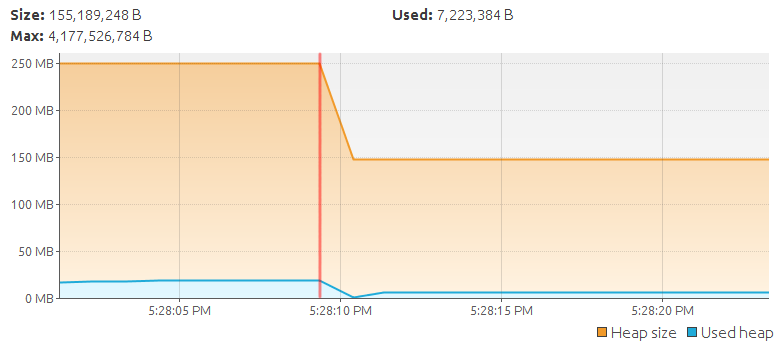
\includegraphics[scale=0.5]{obrazky/heapdump-performed.png}
	\caption{Využití paměti a provedení garbage kolekce před vytvořením dumpu (červeně).}
	\label{obr1}
\end{figure}

\subsection{Zpracování dumpu}
Při zpracování dumpu je nutné zohlednit fakt, že je vyexportovaný kompletní paměťový prostor [TODO zdroj] a nachází se zde tedy i data objektů, které nás nutně nemusí zajímat – typicky knihovny nebo objekty Javy. Toto je možné zohlednit a filtrovat na základě jmenného prostoru (namespace), do kterého objekt patří.

Pro práci nad heapem  (typicky ve formátu HPROF) je možné využít některou z implementací dotazovacího jazyku OQL (Object Query Language).

\subsection{Binární formát dumpu heapu}
Binární formát dumpu Java heapu (\textit{hprof}) má specifikovaný formát, který je popsán v tabulkách \ref{table-hprof-header} a \ref{table-hprof-body}.

\subsubsection{Hlavička}
\begin{table}[ht!]
    \begin{tabularx}{\textwidth}{|l|X|}
        \hline
    \textbf{Velikost} & \textbf{Popis} \\ \hline \hline
    $n + 1$ B & Formát a verze dumpu délky $n$. Velikost není specifikována, pole bytů je ukončeno hodnotou \texttt{null}. \\
    4 B & Velikost identifikátorů. Mohou mít stejnou velikost jako ukazatele hostitelského systému, ale není to nutné. \\
    4 B & Část data (high-order word) z Unix timestampu. \\
    4 B & Část data (low-order word) z Unix timestampu.  \\ \hline                                                                   
    \end{tabularx}
    \caption{Hlavička \texttt{hprof} binárního formátu.}
    \label{table-hprof-header}
\end{table}

\subsubsection{Tělo}
Tělo formátu dumpu je složeno ze sekvence (či pole) položek následujícího formátu.
\begin{table}[ht!]
    \begin{tabularx}{\textwidth}{|l|X|}
        \hline
    \textbf{Velikost} & \textbf{Popis} \\ \hline \hline
    1 B & Tag -- typ záznamu -- viz tabulka \ref{table-hprof-types}. \\
    4 B & Čas -- počet milisekund, které uplynule od Unix timestampu v hlavičce. \\
    4 B & Délka -- počet bytů $n$, které následují a slouží jako obsah záznamu. \\
    $n$ B & Obsah záznamu. \\ \hline                                                                   
    \end{tabularx}
    \caption{Tělo \texttt{hprof} binárního formátu.}
    \label{table-hprof-body}
\end{table}


\subsubsection{Typy záznamů}
Tabulka s tělem obsahuje pole záznamů, v nichž je typ záznamu -- pole \textit{tag}. Celkově je podporováno 13 následujících typů -- z toho většina má ještě, jako obsah, další -- více či méně komplexní -- strukturu.
\begin{table}[ht!]
    \begin{tabularx}{\textwidth}{|l|X|}
        \hline
    \textbf{Tag} & \textbf{Popis} \\ \hline \hline
    0x01 & Dump řetězce. \\
    0x02 & Načtení třídy. \\
    0x03 & Odstranění (ve smyslu opaku načtění) třídy. \\
    0x04 & Rámec (položka) stacku. \\
    0x05 & Stack trace. \\
    0x06 & Alokace. \\
    0x07 & Souhrn některých hodnot heapu. \\
    0x0A & Počátek vlákna. \\
    0x0B & Konec vlákna \\
    0x0C/0x1C & Heap dump, respektive heap dump segment. \\
    0x2C & Konec heap dumpu. \\
    0x0D & CPU vzorkování. \\
    0x0E & Hodnoty některých nastavení. \\ \hline                                                                   
    \end{tabularx}
    \caption{Typy položek \texttt{hprof} binárního formátu.}
    \label{table-hprof-types}
\end{table}

\subsubsection{Typy dumpovaných hodnot}
Některé z výše zmíněných typů (které jsem dále nerozepisoval) už obsahují přímo data programu (ať už uživatelská nebo pomocná). Proto jsou definovány typy těchto dat, které jsou shrnuty v tabulce \ref{table-hprof-data-types}. Pole jsou definována pomocí řetězcu s jejich názvem tak, jak by se objevily v Javě, tedy např. \texttt{int[][]}.
\begin{table}[ht!]
    \begin{tabularx}{\textwidth}{|l|X|}
        \hline
    \textbf{Označení} & \textbf{Datový typ} \\ \hline \hline
    2 & \texttt{Object}. \\
    4 & \texttt{Boolean}. \\
    5 & \texttt{Char}. \\
    6 & \texttt{Float}. \\
    7 & \texttt{Double}. \\
    8 & \texttt{Byte}. \\
    9 & \texttt{Short}. \\
    10 & \texttt{Int}. \\
    11 & \texttt{Long}. \\ \hline
    \end{tabularx}
    \caption{Datové typy položek \texttt{hprof} binárního formátu.}
    \label{table-hprof-data-types}
\end{table}

% =====================================================================================================================================================================================



\chapter{Analýza paměti}

Paměť je možné analyzovat za běhu programu nebo z jejího snímku -- reprezentace paměti v určitém okamžiku běhu programu.

\section{Analýza za běhu programu}
\label{runtime-analysis}
Během běhu programu lze analyzovat aktuální obsah paměti -- \zkratka{GC} koneckonců nedělá nic jiného. Problémem tohoto přístupu je ovšem dopad na výkon. I samotný \zkratka{GC}, ať už umožňující současný běh kódu nebo \textit{stop-the-world}, má výrazný dopad na výkon oproti jazykům či běhovým prostředím bez něj \cite{gc}. Navíc, běh \zkratka{GC}, stejně tak jako režie běhu samotného prostředí, jsou v drtivé většině případů v maximální možné míře optimalizovány, aby byl dopad na výkon samotného programu co nejmenší a jeho běh co nejrychlejší. Mohou využívat celou řadu nízkoúrovňových optimalizací, kterých -- v některých jazycích, včetně Javy -- dosáhnout prakticky nemůžeme. Z toho můžeme usoudit, že dopad analýzi paměti programu za jeho běhu by byl přinejmenším takový, jako dopad běhu \zkratka{GC}; pravděpodobně však výrazně vyšší. Stejně tak musíme uvažovat, že běh naší analýzy -- ať už pouze za účelem sběru dat pro pozdější zpracování -- bude výrazně složitější (či výkonově náročnější), než běh \zkratka{GC}.

Dalším důvodem pro vyhnutí se analýze za běhu programu je povaha řešeného problému a tedy implementovaného algoritmu. Protože potřebujeme provádět hloubkovou analýzu (všech či vybraných) objektů programu, jejich neustálá změna by tuto analýzu za běhu programu učinila nemožnou -- z tohoto důvodu vyžadují různé implementace \zkratka{GC} \textit{stop-the-world}. Respektive bychom se nemohli vyhnout eventuálním falešně negativním či positivním hlášením -- to si jednoduše můžeme představit. Jestliže s každým cyklem analýzy zpracujeme jeden objekt a během toho dojde ke změně dat některého z dalších objektů, pak by algoritmus zahlásil při zpracování dalších objektů falečně pozitivní nález. V žádném časovém okamžiku neexistovaly dva objekty se stejnými daty, algoritmus by je tak přesto označil.


\begin{figure}[h]
	\centering
	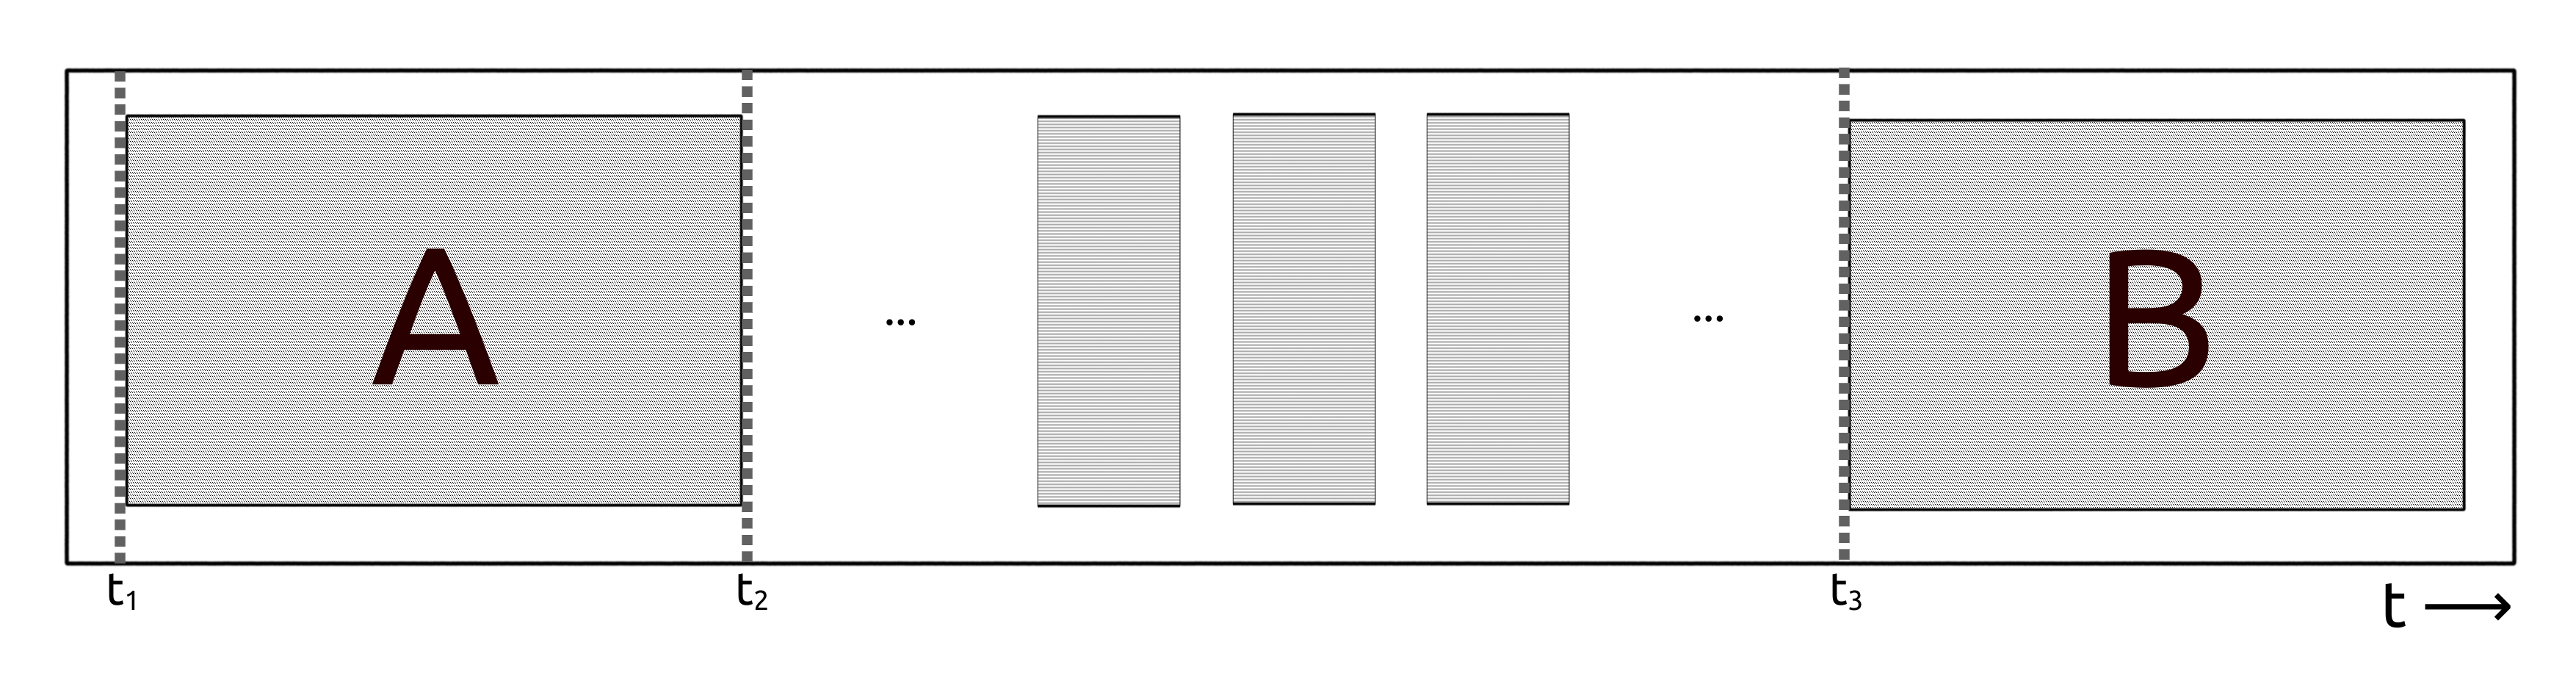
\includegraphics[scale=0.5]{obrazky/runtime-analysis.png}
	\caption{Problém analýzy paměti za běhu programu.}
	\label{obrRuntimeAnalysis}
\end{figure}



% =====================================================================================================================================================================================



\chapter{Optimalizace užití paměti}

Jak již bylo zmíněno v úvodu, využití paměti lze optimalizovat na několika úrovních. Vzhledem k tématu této práce se při uvažování optimalizací omezíme pouze na běžící Java aplkaci. Eliminaci případných zbytečných knihoven, frameworků a nástrojů se věnovat rovněž nemusíme. Analyzovat procentuální využití nabízených funkcí knihovny by mohlo být zajímavé, nicméně tento typ zbytečného užívání paměti nelze přímo označit za memory waste.

Můžeme tedy omezit samotné využití objektů -- zvážit, zda je potřebujeme, případně zda neexistuje vhodnější způsob či struktura pro jejich uchovávání. Jejich alokaci v paměti bychom rovněž meli omezit na nejkratší možnou dobu, po kterou si budeme jisti jejich využitím. Nicméně i zde je vhodné najít vhodný poměr mezi optimalizací a zbytečným úklidem objektu, který za několik okamžiků znovu budeme vytvářet.

Nejpřímějším způsobem optimalizace užití paměti se může jevit odstranění objektů, které už nejsou zapotřebí a nikdo je tedy nevlastní. Takové objekty nicméně nemusíme v naší optimalizaci uvažovat. O jejich uvolnění z paměti se postará \zkratka{GC}. Této vlastnosti jazyku tedy můžeme využít a nepotřebné objekty ručně odstraňovat -- nastavit je jako \texttt{null}. K jejich uvolnění dojde i při opuštění aktuálního prostoru -- oboru platnosti lokální proměnné. K takovému uvolnění nicméně nedochází přímo zapomocí analýzy \zkratka{GC}, ale díky uložení lokálních proměnných v stacku, z kterého jsou při opuštění bloku odstraněny.



% =====================================================================================================================================================================================



\chapter{Java Virtual Machine}
Program napsaný v Javě běží typicky v některé z implementací \zkratka{JVM}. \zkratka{JVM} je program, který slouží jako běhové prostředí pro uživatelský kód -- vykonává jeho instrukce a slouží tak jako prostředník mezi ním a operačním systémem (respektive jako interpret jeho kódu, který následně překládá do jiného jazyka, typicky strojového kódu dané architektury či platformy). \zkratka{JVM} je možné si představit jako virtuální počítač -- má vlastní instrukční sadu a na základě ní provádí operace nad pamětí. Díky tomu je možné jej, v případě potřeby, implementovat i jako CPU -- taková hardwarová implementace se nazývá \textit{Java procesor}. 

\zkratka{JVM} nemá ponětí o existenci Javy jako jazyku. Vidí pouze výsledek kompilace do bytecodu (viz dále), což je posloupnost operací z výše zmíněné instrukční sady. Jako analogii je možné zmínit instrukční sadu CPU a strojový kód -- CPU také netuší, jaký vyšší programovací jazyk je původcem strojového kódu, a při podobné implementaci kompilátoru dvou jazyků by to ani neměl šanci zjistit. Stejně tak se chová \zkratka{JVM} a bytecode -- ostatně existují i další jazyky na platformě \zkratka{JVM}, za všechny můžu jmenovat třeba populární Kotlin \cite{jvms-jvm}.

Některé implementace \zkratka{JVM} umožňují přímý překlad do strojového kódu bez potřeby interpretace, např. GraalVM \cite{graalvm}. V takovém případě hovoříme o tzv. \zkratka{AOT} přístupu, místo \zkratka{JIT} postupu implementovaného v moderních verzích častěji používaných \zkratka{JVM}, např. HotSpot od společnosti Oracle [TODO zdroj, že HS používá JIT].

\zkratka{JVM} se stará o načtení kódu ze souboru \texttt{.class}, dále o jeho verifikaci, spuštění a zároveň poskytuje tomuto kódu prostředí, v rámci kterého může běžet.

\section{Java Bytecode}
Java využívá dvoufázový překlad, tj. samotný zdrojový kód vytvořený programátorem je nejprve přeložen do \textit{bytecodu} (či česky bytekód). Bytecode je (či by měl být) platformě nezávislý soubor instrukcí, který následně \zkratka{JVM} vykoná v prostředí architektury a platformy, na které je spuštěn. To znamená, že zdrojový kód v jazyce Java (či kompatibilních jazycíc využívajících stejné prostředí, např. Kotlin), uložený typicky v souboru \texttt{.java}, je přeložen do bytecodu -- typicky s typu \texttt{.class}. Takové soubory je následně, obecně vzato, možné přenést na jinou platformu či architekturu a jestliže se zde nachází kompatibilní \zkratka{JVM}, je možné jej bez úpravy na daném systému vykonat a tedy program spustit. Bytecode se může přenášet formou klasických jednotlivých souborů \texttt{.class} či v zabalené formě, tj. archiv typu \texttt{.jar} (což je de facto pouze zip archiv s předem danou strukturou a volitelně přidanými informacemi -- manifestem, metadaty, podpůrnými soubory (\textit{resources})).

\section{Class loader}
Jak už jsem zmínil, \zkratka{JVM} se stará o načítání dat ze souboru \texttt{.class}. Konkrétně se o toto načítání stará objekt nazvaný \textit{class loader}. Ten, typicky, načítá třídy ze souborového systému, konkrétně z cesty (nebo z více cest) definované v proměnné \texttt{CLASSPATH}. Nicméně, díky tomu, že koncept class loaderů je poměrně abstraktní, je možné načítat třídy například přes síť, z paměti nebo je dynamicky vytvářet za běhu programu dle potřeby. Každá načtená třída (konkrétně objek typu \texttt{Class}) obsahuje referenci na objekt class loaderu, který ji zavedl do programu -- konkrétně jej lze obdržet pomocí metody \texttt{getClassLoader()} (v případě primitivních typů vrací \texttt{null}). \texttt{ClassLoader} je definovaný jako abstraktní třída, lze tedy definovat vlastní loadery dle potřeby. 

Pokud \texttt{JVM} narazí na třídu, podívá se do setu načtených tříd. Jestliže se tam nachází, vezme ji (instanci třídy \texttt{Class}) a použíje. Pokud ne, požádá o její načtení. Systém class loaderů funguje na principu delegování v následujícím pořadí (typicky, pokud jej neupravíme), jak zobrazuje obrázek \ref{obr-class-loader} \cite{class-loader} \cite{class-loader-hierarchy}. V případě, že třídu žádný z boot loaderů nenalezne, je produkována výjimka \texttt{ClassNotFoundException}. 

\begin{enumerate}
	\item Aplikace požádá \textit{Application class loader} o načtení třídy.
	\item Ten zavolá \textit{Extension class loader}.
	\item \textit{Extension class loader} zavolá \textit{Bootstrap class loader}.
	\item \textit{Bootstrap class loader} funguje v rámci výchozích \textit{JDK} a \textit{JRE} knihoven. Pokud třídu nalezne, tak ji vrátí. V opačném případě volá zpět \textit{Extension class loader}.
	\item \textit{Extension class loader} se podívá v rámci rozšíření \textit{ext} Javy. V případě neúspechu volá \textit{Application class loader}.
	\item \textit{Application class loader} načítá třídy z \texttt{CLASSPATH} (a třídy specifikované v Manifestu atd.)
\end{enumerate}

\begin{figure}[ht!]
	\centering
	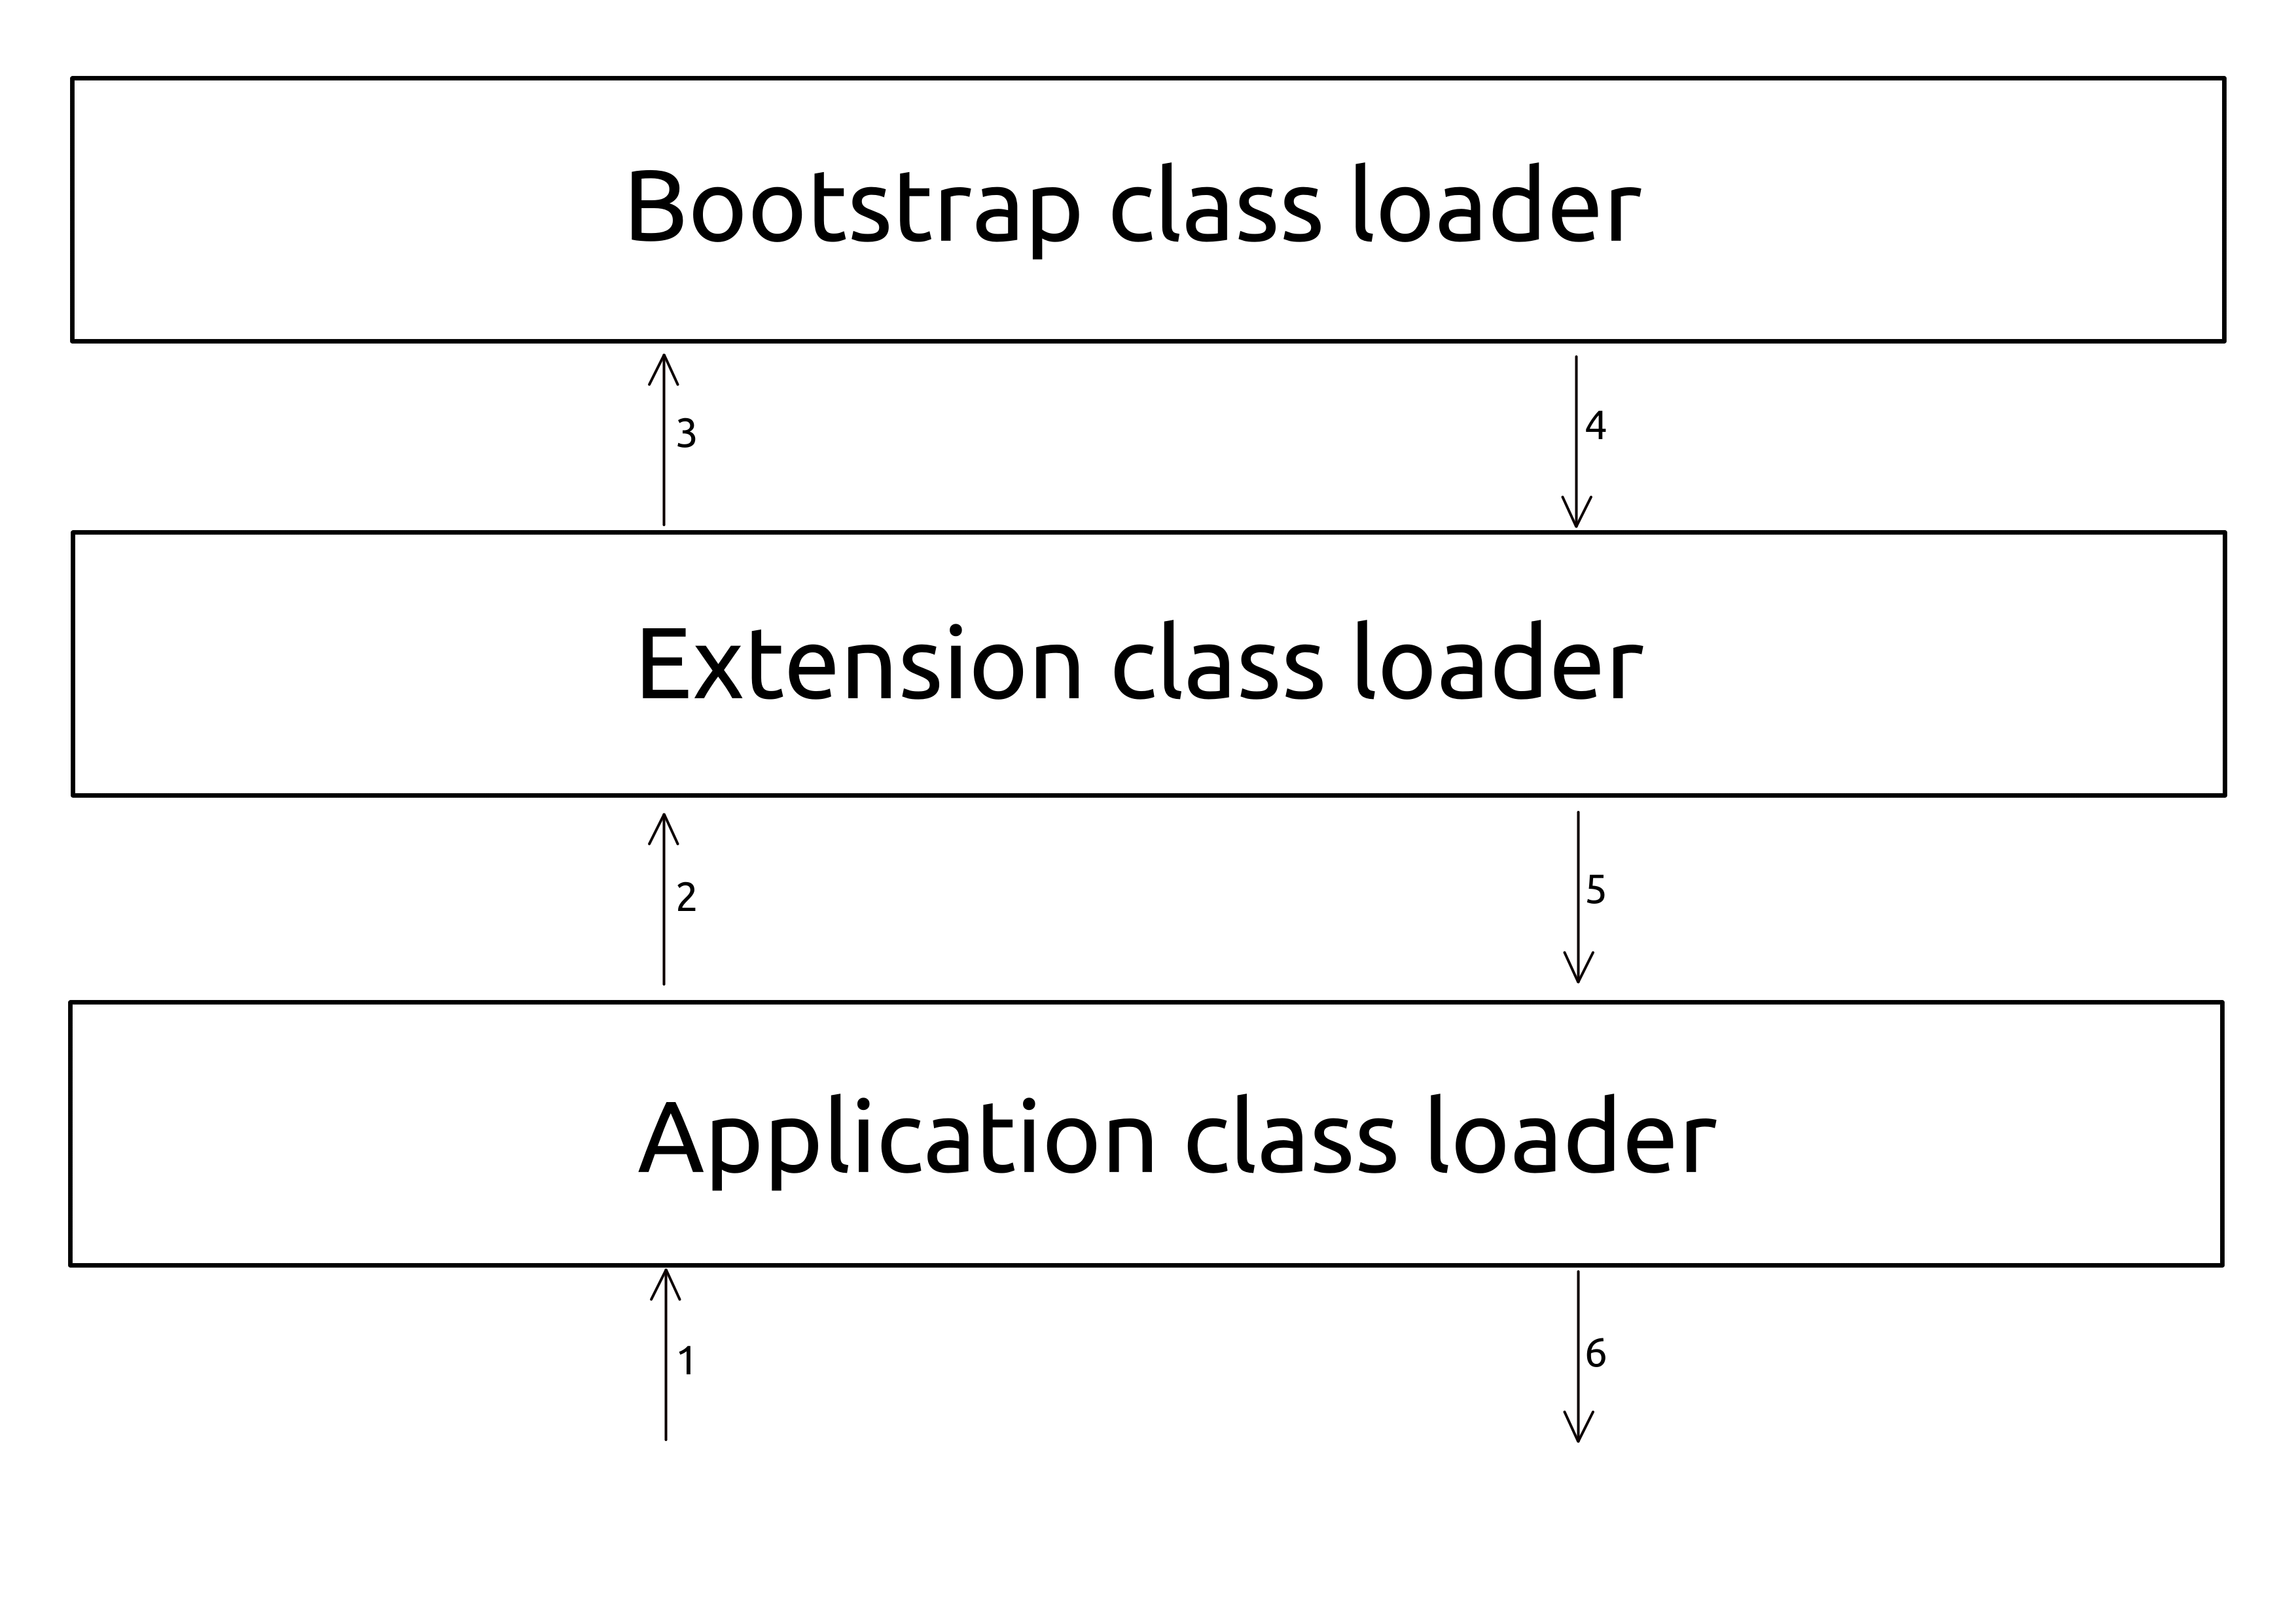
\includegraphics[scale=0.5]{obrazky/class-loader.png}
	\caption{Postup volání hierarchie class loaderů.}
	\label{obr-class-loader}
\end{figure}



% =====================================================================================================================================================================================



\chapter{Existující nástroje pro analýzu heapu}
\label{existing-solutions}
Analýza dumpu -- ať už manuální či automatická -- je využívána v případech, kdy nám debugování na úrovni kódu už nestačí a potřebujeme se podívat, jakým způsobem se program chová na pozadí. Některé typy problémů navíc pomocí debuggeru odhalíme jen těžko (nebo vůbec) a musíme tak zvolit nízkoúrovnější způsob, který dokáže odhalit problém napříč více částmi aplikace. Rovněž je taková analýza vhodná v okamžiku, kdy dojde k pádu (zejména v důsledku nedostatku paměti), kdy chceme zjistit příčinu pádu \uv{post mortem}. Můžeme tak odhalit problematické místo v programu a podrobná analýza nám tak umožní problém opravit.

TODO přidat licence a další info.

\section{Eclipse MAT}
IBM Eclipse Memory Analyser Tooling je open source nástroj pro analýzu Java paměti. Po spuštění umožňuje otevřít již vygenerovaný dump Java heapu, umí jej ale i vytvořit. V rámci analýzy nabízí 2 konkrétní volby – analýzu memory leaků a memory bloatu – tj. neefektivního využití paměti a zbytečného plýtvání. 

MAT se analýzou memory bloatu přibližuje zamýšlenému výsledku této práce, bohužel ale nenabízí kompletní funkcionalitu v této oblasti. Omezuje se pouze na efektivní práci s řetězci (kterou už obsahuje Java, respektive JVM v základu, viz \ref{java-strings}) a dalšími základnímu typy, např. Map. Cílem práce je ale zpracování všech možných objektů, tato funkcionalita by se tak dala případně rozšířit.

Nástroj je založený na platformě Eclipse RCP (Rich Client Platform), respektive OSGi. Díky tomu je poměrně snadno rozšiřitelný, což je ale vyváženo velkým rozsahem aplikace, který vývoj a rozšíření naopak lehce komplikuje. Buildovacím nástrojem je zde Maven.

\subsection{Základní informace}

\begin{description}
    \item[Licence] Eclipse Public License 1.0
    \item[Jazyk] Java
    \item[Zdrojový kód] \url{https://git.eclipse.org/c/mat/org.eclipse.mat.git} 
    \item[Výhody] Již obsahuje základní funkcionalitu, která by se dala využít pro potřeby splnění zadání této práce.
    \item[Nevýhody] Jedná se o velmi obsáhlý projekt, jehož úprava není jednoduchá a pro potřeby této práce je využitelný malý zlomek jeho funkcionality.
\end{description}

\begin{figure}[ht!]
	\centering
	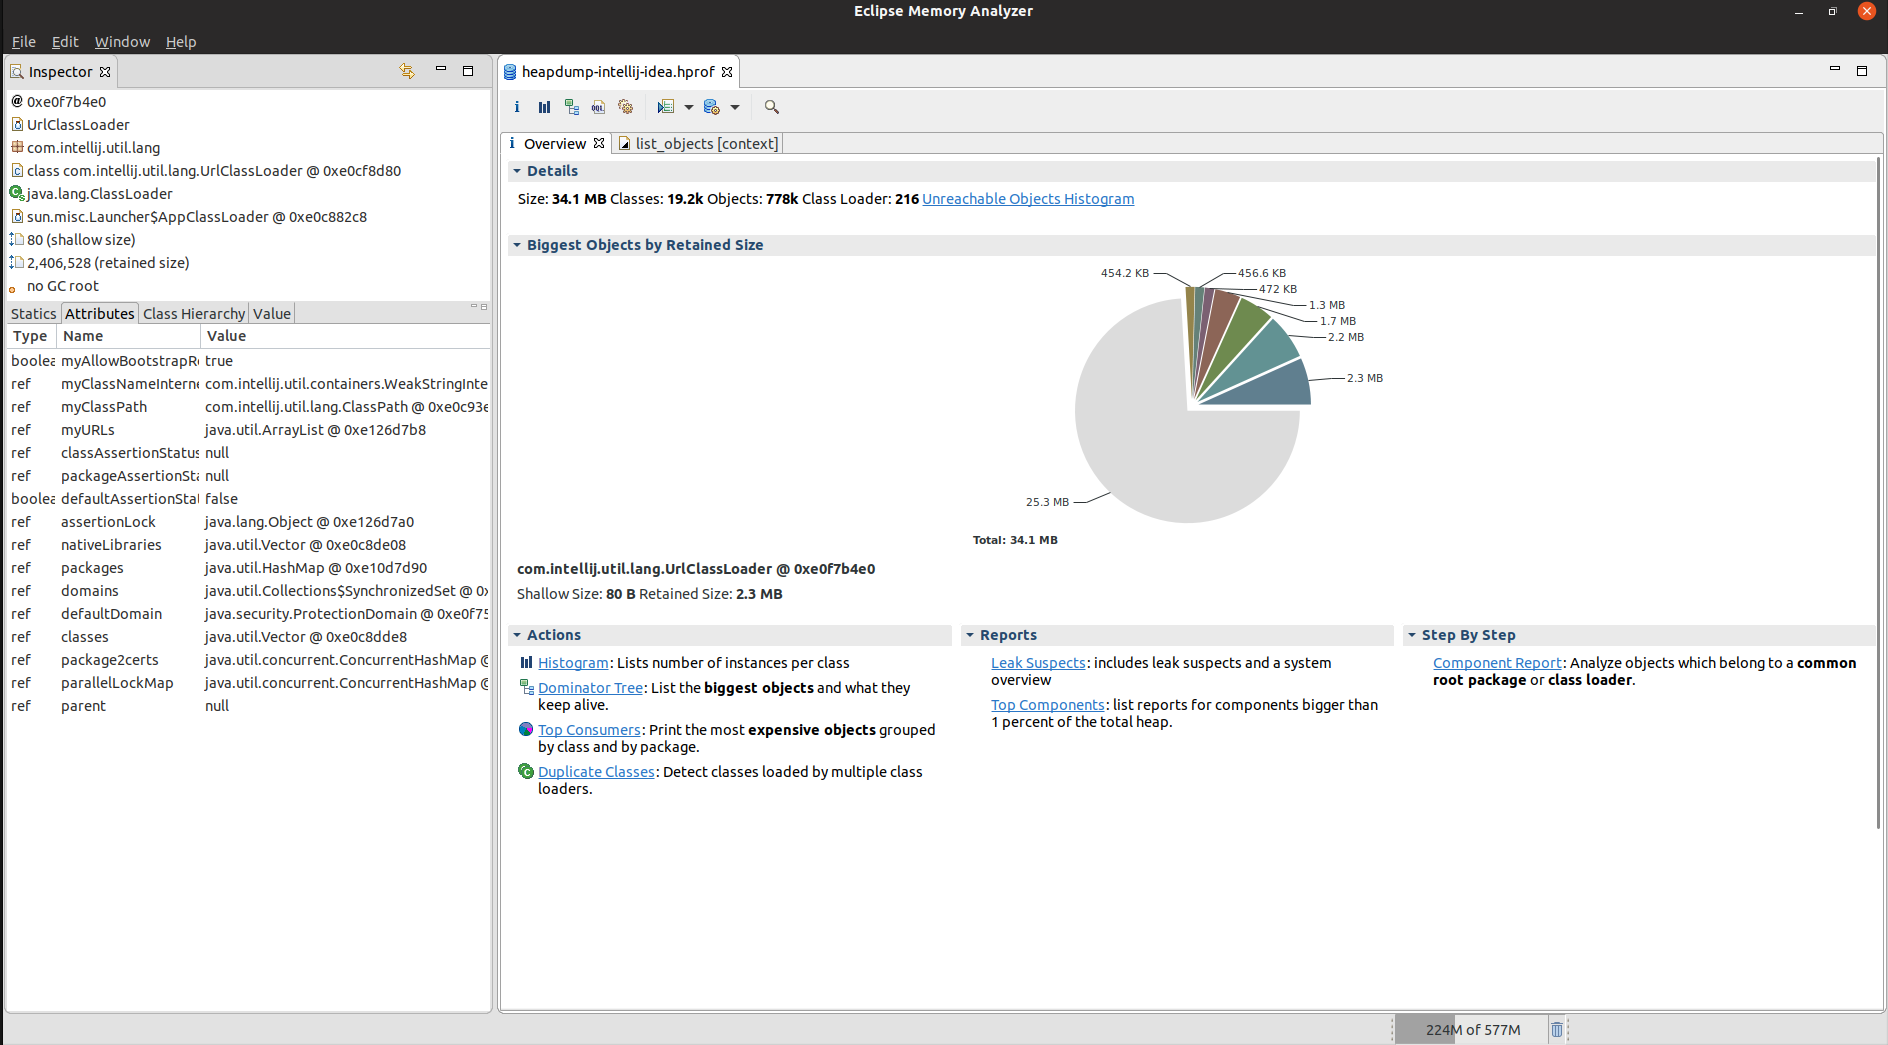
\includegraphics[scale=0.3]{obrazky/mat.png}
	\caption{Rozhraní Eclipse MAT}
	\label{obr-eclipse-mat}
\end{figure}


\section{VisualVM}
Open source profiler pro Java platformu. Patří mezi nejpoužívanější profilery, respektive nástroje pro analýzu výkonu v Javě.

Po spuštění nabízí klasické funkce typické pro profilery, tj. využití paměti, zatížení CPU, počet objektů a vláken a podobné statistiky. Kromě toho obsahuje celou řadu dalších funkcí, jako provedení garbage kolekce (její vyžádání, explicitně vyvolání GC není možné) nebo vytvoření heap dumpu.

Požadovanou funkcionalitu VisualVM v zásadě neposkytuje, umožňuje pouze k nahlédnutí tabulku s informacemi – kolik bylo vytvořeno instancí jaké třídy, respektive jimi okupovanou paměť. V programu existuje podpora pro OQL syntaxi, což je možné využít, nicméně tento přístup nelze považovat za dostačující.

Pro build je využíván nástroj Ant a v současné době je vyžadována Java verze 7 a vyšší.

\subsection{Základní informace}

\begin{description}
    \item[Licence] GPLv2 + CE
    \item[Jazyk] Java
    \item[Zdrojový kód] \url{https://github.com/oracle/visualvm} 
    \item[Výhody] Populární nástroj, jehož vývoj je (v době psaní této práce) stále velmi aktivní.
    \item[Nevýhody] Stejně jako v případě Eclipse MAT velmi rozsáhlý a komplikovaný projekt. Kromě předzpracování dumpu neposkytuje žádnou požadovanou funkcionalitu.
\end{description}

\begin{figure}[ht!]
	\centering
	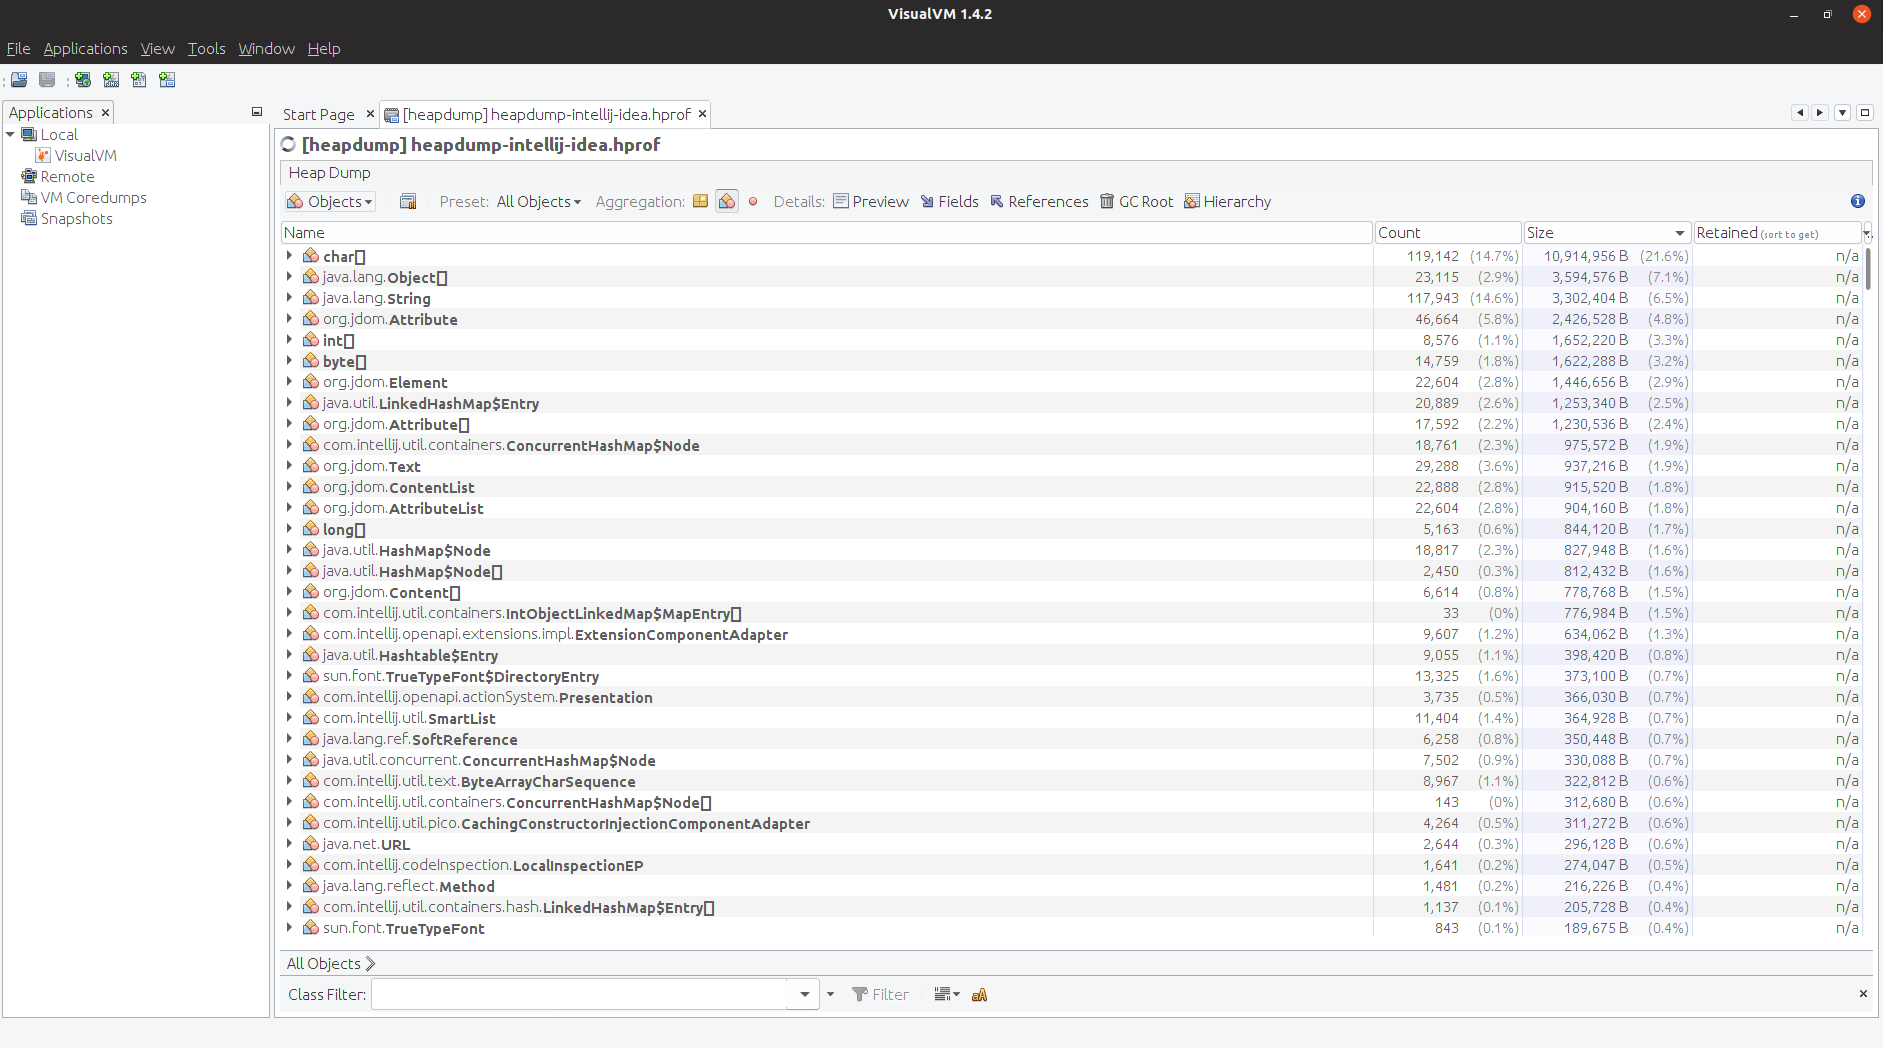
\includegraphics[scale=0.3]{obrazky/visualvm.png}
	\caption{Rozhraní VisualVM}
	\label{obr-visualvm}
\end{figure}

\section{Java Mission Control}
Nástroj poskytovaný přímo spolu s distribucí Oracle JVM od verze 7 (konkrétně 7 Update 40 – 7u40), což je jeho výhodou. Mezi jeho možnosti patří např. využití paměti jednotlivými součástmi Java paměti a také umožňuje zobrazit jednotlivé instance objektů, nicméně neumožňuje jejich další analýzu.

\subsection{Základní informace}

\begin{description}
    \item[Licence] Universal Permissive License (UPL), Version 1.0 nebo BSD
    \item[Jazyk] Java
    \item[Zdrojový kód] \url{https://hg.openjdk.java.net/jmc} 
    \item[Výhody] Nástroj je součástí JDK, jeho rozšíření (formou pluginu) by mohlo výrazně přispět k použitelnosti vytvořené aplikace.
    \item[Nevýhody] Neumí zpracovávat HPROF soubory.
\end{description}

\begin{figure}[ht!]
	\centering
	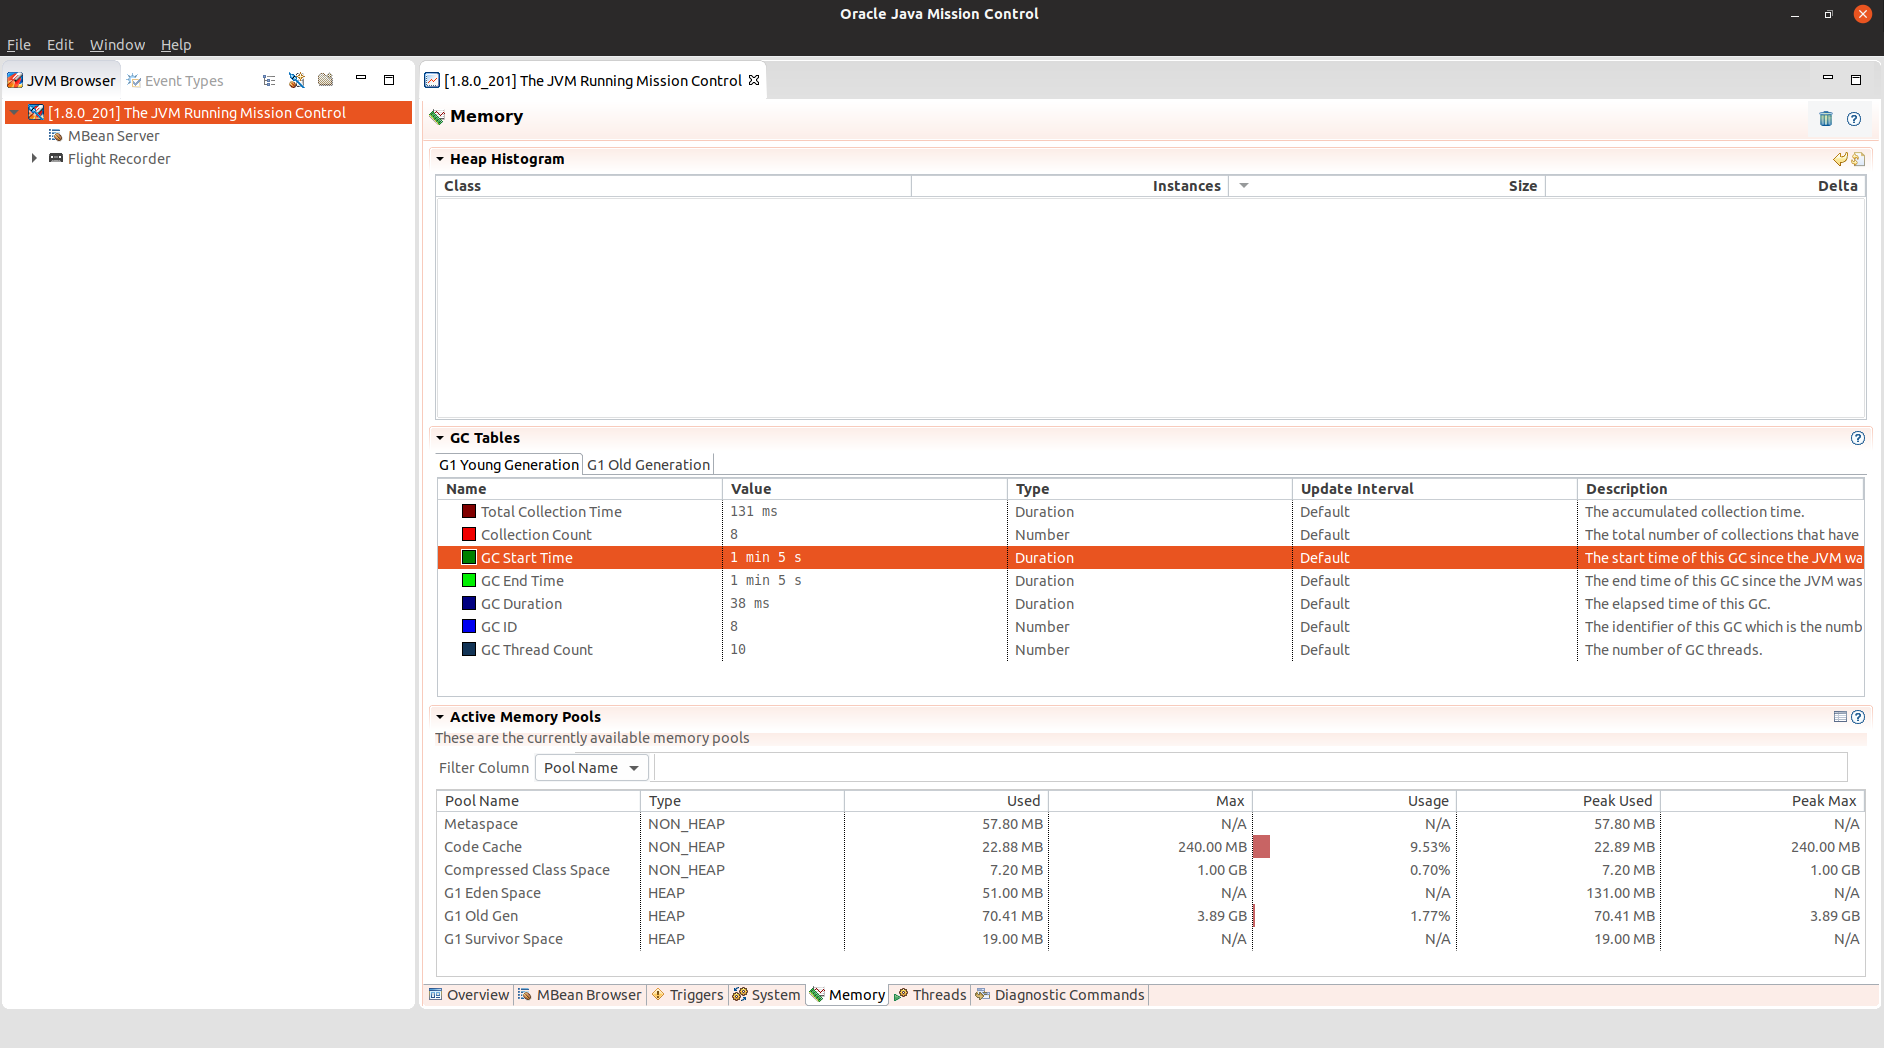
\includegraphics[scale=0.3]{obrazky/jmc.png}
	\caption{Rozhraní Java Mission Control}
	\label{obr-jmc}
\end{figure}

\section{JProfiler}
Komerční profiler, přesto velice používaný. Standardní licence stojí v době psaní 409 euro, akademická potom 179 euro. Je možné zažádat o licenci pro open source produkty, nicméně ta je podmíněna již vydanou verzí a existující webovou stránkou, což činí jakékoliv použití tohoto profileru v rámci práce nepraktickým. Profiler je používán především v komerční sféře, díky svým možnostem a dle výše uvedeného testu i nejvyšší úspěšností v odhalování bugů.

\clearpage
\subsection{Základní informace}

\begin{description}
    \item[Licence] Proprietární -- placení software
    \item[Jazyk] Java
    \item[Zdrojový kód] Není opensource
    \item[Výhody] Komeční nástroj, velké možnosti, obsahuje porovnání základních objektů.
    \item[Nevýhody] Není zdarma.
\end{description}

\begin{figure}[ht!]
	\centering
	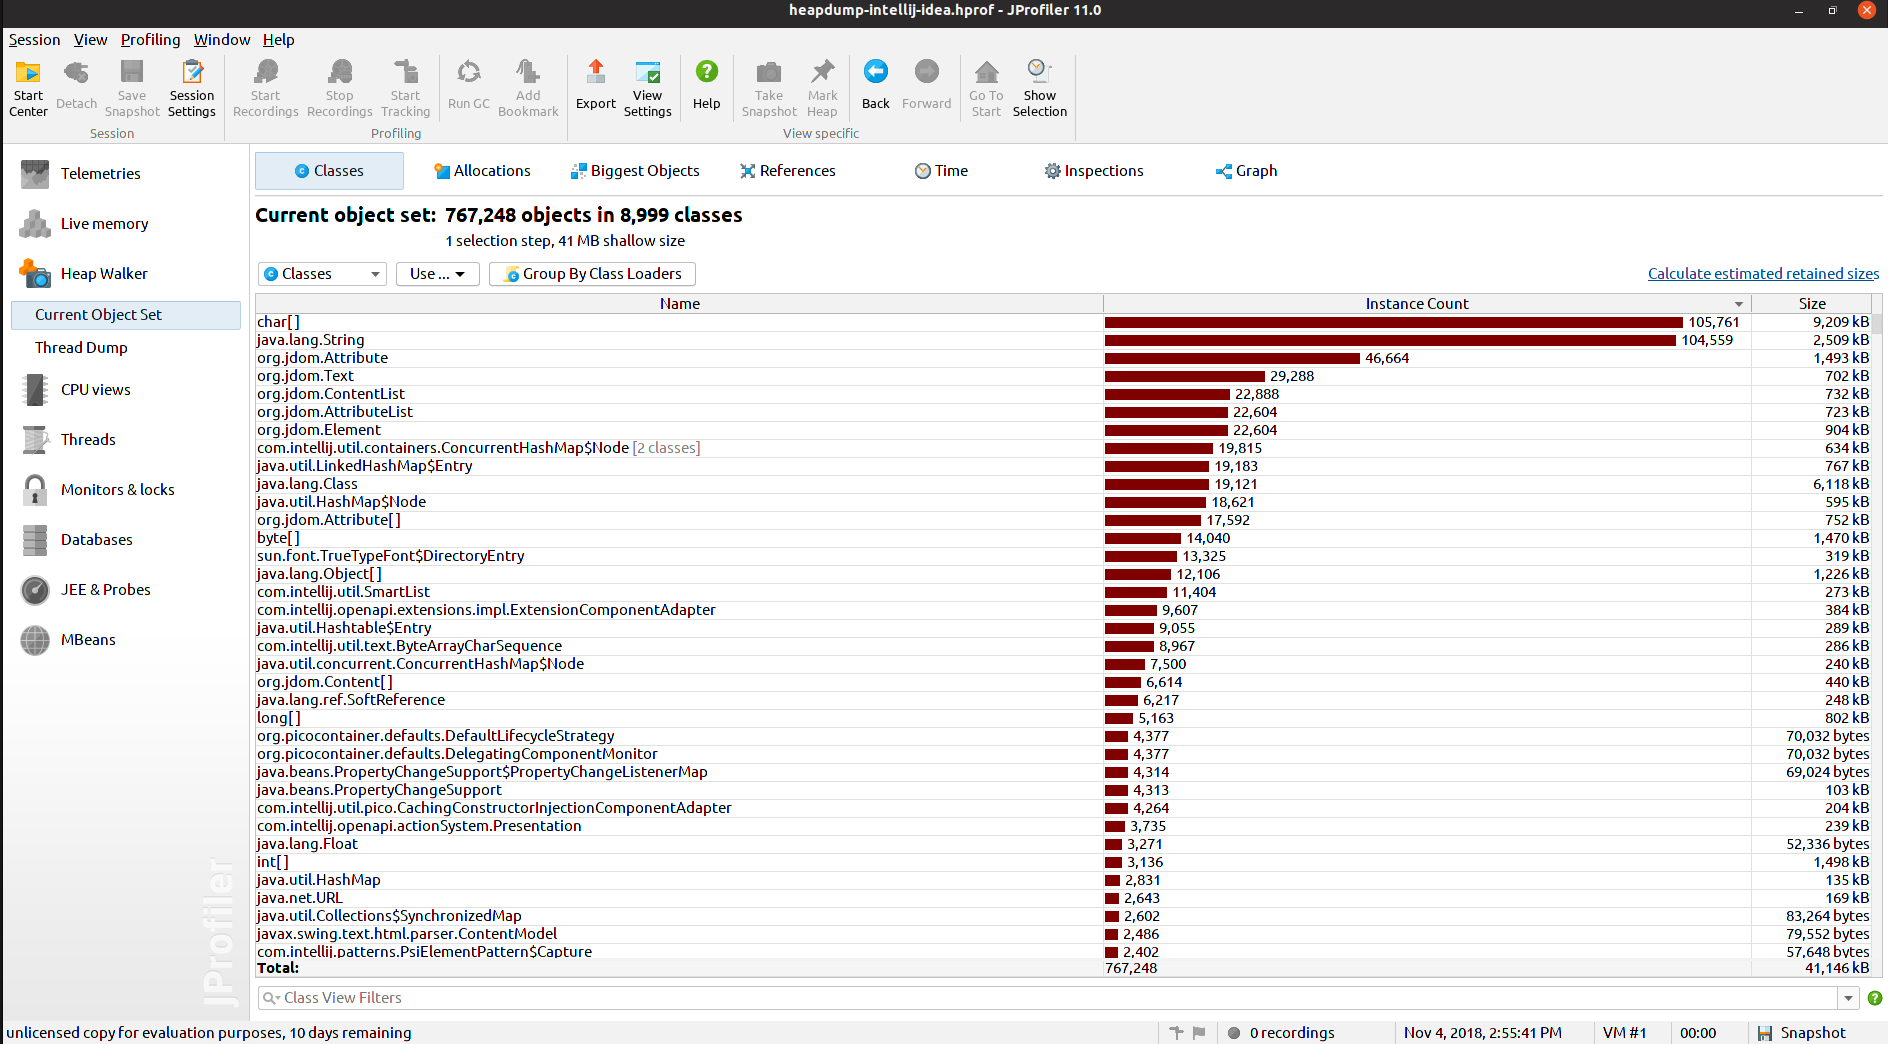
\includegraphics[scale=0.3]{obrazky/jprofiler.png}
	\caption{Rozhraní JProfileru}
	\label{obr-jprofiler}
\end{figure}

\section{JHAT}
Nástroj, který je přímou součásti distribuce Oracle JVM od verze 6. Nebyl nikdy oficiálně podporován a od počátku byl označen jako experimentální nástroj, z těchto důvodů byl tedy v Javě 11 naprosto odstraněn \cite{jep241}\cite{java11migration}. V rámci verzí Javy, které jej obsahují, ho lze využít jako \zkratka{CLI} aplikaci, která dokáže dump vytvoření pomocí např. \textit{JMAP} otevřít. Následně vytvoří webový server, jehož prostřednictvím poskytuje data získaná ze zpracovaného dumpu. Tato data je možné si poté zobrazit pomocí webového prohlížeče; zajímavým příkladem možného využití je následné rozparsování těchto dat jakožto formátu HTML a jejich další využití. Program je tedy možné využít jako prostředníka pro zpracování \cite{jhat}. Kromě \uv{prostého} zobrazení webové stránky umí \textit{JHAT} rovněž poskytovat zpracování pomocí jazyka \zkratka{OQL}.

\subsection{Základní informace}

\begin{description}
    \item[Licence] SUN PUBLIC LICENSE Version 1.0
    \item[Jazyk] Java
    \item[Zdrojový kód] \url{https://download.java.net/openjdk/jdk8/}
    \item[Výhody] Byl součástí starších verzí JDK, nyní už není.
    \item[Nevýhody] Již není podporován. Nabízí jen základní funkcionalitu.
\end{description}

\begin{figure}[ht!]
	\centering
	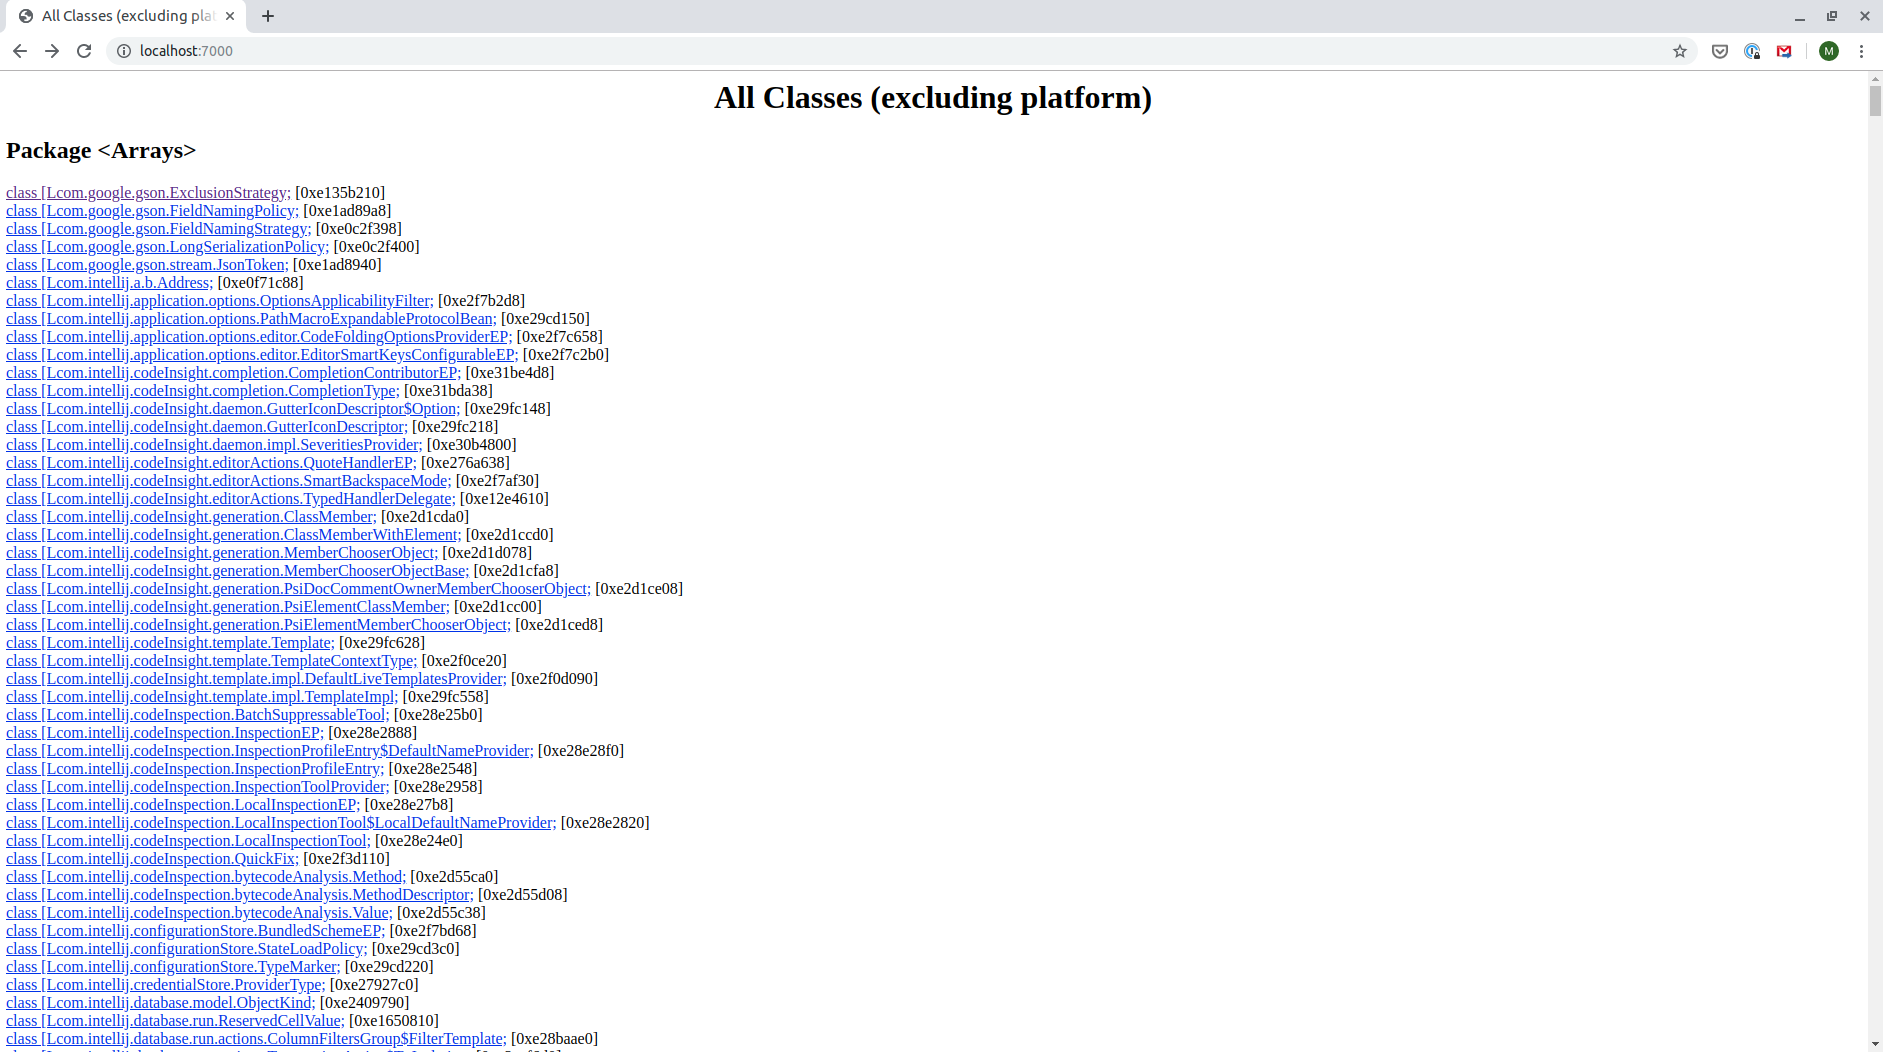
\includegraphics[scale=0.3]{obrazky/jhat.png}
	\caption{Rozhraní JHAT}
	\label{obr-jhat}
\end{figure}

\section{OQL}
\zkratka{OQL} zmíním i jako samostatný způsob zpracování. Jedná se o jazyk, který slouží pro obecnou manipulaci s objekty, resp. s objektovými dokumenty \cite{odmgoql}\cite{oql}. Na první pohled si nelze nevšimnou jeho podobnosti s dotazovým jazykem SQL. Neomezuje se tedy pouze na zpracování Java heapu (či obecně paměti), ale je standardem, který pro tento účel lze využít. Z toho je možné usoudit, že standard jako takový pro zpracování nestačí -- je nutné využít některou z jeho implementací, která takové rozhraní přístupu k Java heapu umožňuje. Jednou z nich je právě výše zmíněný \textit{JHAT}.

V příkladu \ref{example-oql} je možné vidět práci s OQL.

\begin{lstlisting}[caption={Příklad OQL}, label={example-oql}, frame={single}, language={SQL}]
select s 
from java.lang.String s 
where s.value.length >= 100
\end{lstlisting}

\section{Knihovny}
Knihovny představují způsob přístupu k problému, který by nevyžadoval zásah do již existujícího kódu, ale spíše jeho využití. A to tak, že se starají o jednu specifickou část, kterou tak není nutné implementovat znovu. I výše zmíněné aplikace lze považovat z pohledu API za knihovny, nicméně již vyžadují dodržení jejich struktury a zorientování se v, často velmi rozsáhlém, existujícím kódu.

% =====================================================================================================================================================================================



\chapter{Možnosti analýzy}

\section{Rovnost objektů}
Rovnost dvou či více objektů se dá definovat a zjišťovat různými způsoby. Je ale nutné si uvědomit, že v nejhorším případě, tj. pokud chceme najít všechny nadbytečné kopie každého objektu, je složitost této operace $O(2^n)$. Bylo by tedy vhodné se zamyslet, zda neexistuje způsob, jak počet porovnání snížit, případně navrhnout jednoduchou heuristiku, která by dokázala rychle ohodnotit, zda má vůbec smysl pokračovat v podrobnějším porovnání. V následujících případech tedy uvažujme objekty $A$, $B$, jejich třídy $C_A$ a $C_B$ a proměnné obou instancí $F_A^0..F_A^n$, respektive $F_B^0..F_B^n$. Hodnotu dané instanční proměnné definujeme jako $V(F)$. Pro potřeby algoritmu předpokládejme, že jsou tyto proměnné v určitém, předem očekávatelném pořadí, např. podle abecedy dle jejich názvu (nebo dle Unicode kódu pro speciální znaky).

První nápovědou samozřejmě může být porovnání tříd obou objektů -- $C_A$ a $C_B$. Pokud platí $C_A = C_B$, zřejmě má smysl se porovnáváním dále zabývat. V případě jejich nerovnosti není ale možné další porovnání zavrhnout, porovnat je nutné (či možné) i jejich rodiče. V případě dědičnosti dvou tříd nelze automaticky vyloučit -- pokud potomek k rodičovské třídě nepřidává žádná data, pouze funkcionalitu, pak se z pohledu dat v paměti objekty rovnají, i když jsou sémanticky odlišné.

Definujeme-li tedy funkci pro zjištění přímého rodiče $P(C)$, potom rovnost tříd (z pohledu jejich dat) lze vyjádřit jako

\begin{equation}
    E_C(C_A, C_B) \Leftrightarrow C_A = C_B \vee E_C(P(C_A), C_B) \vee E_C(C_A, P(C_B)).   
\end{equation}

Samozřejmě je nutné definovat i zastavovací podmínku, v případě Javy by tedy jeden z parametrů nesměl být třída typu \textit{Object}. Formálně je tedy možné tuto rovnost definovat i jako množinu

\begin{equation}
E_C^{*}(C_A, C_B)= P_c(C_A) \cap P_c(C_B) \notin \emptyset,
\end{equation}

kde $P_c(C)$ je množina třídy samotné a všech jejich rodičů bez “univerzálního předka” všech tříd, v tomto případě \textit{Object}:

\begin{equation}
P_c(C) = \{C, P(C), P(P(C)), \dots, Object\} \setminus Object.
\end{equation}

Tím máme nastavnu podmínku nutnou -- bez rovnosti (tak, jak je výše definována) tříd nemá smysl porovnávat objekty. Nyní se můžeme zaměřit na porovnávání objektů a jejich proměnných samotných. Vzhledem k tomu, že máme zaručenu rovnost tříd, můžeme očekávat zhruba stejnou strukturu, názvy a typy instančních proměnných. Nicméně nemůžeme očekávat přímou rovnost těchto parametrů, díky tomu, jak jsem výše zadefinoval rovnost proměnných. Proto platí:

\begin{equation}
F_A \subset F_B \vee F_A \subset. F_B 
\end{equation}

Naším cílem je ovšem porovnání rovnosti. Musí tedy platit:

\begin{equation}
\|F_A\| = \|F_B\|.
\end{equation}

Tato operace je pouhé porovnání dvou celočíselných hodnot (plus pravděpodobně zjištění velikosti pole), což je zanedbatelná operace, která algoritmus nezpomalí. Tímto je zajištěno, že porovnávané objekty patří pod stejnou třídu či jejího potomka, který nepřidává žádné instanční proměnné, tj. je z pohledu paměti zaměnitelný. To samozřejmě neznamená, že je stejný z pohledu sémantiky či funkcionality; to je však cena za to, že hledáme maximální možnou úsporu. Toto je ovšem funkcionalita, která je jednoduše regulovatelná, tj. v algoritmu je možnost přidat parametr, který bude ovlivňovat způsob porovnávání rovnosti tříd a případně zajistí, že takto budou označeny pouze třídy skutečně stejné, bez ohledu na dědičnost.

Nyní jsou tedy objekty stejných (dle výše definovaných měřítek) tříd a mají stejný počet proměnných. Vzhledem k tomu, že proměnnou nelze při dědičnosti odebrat ani pozměnit, můžeme předpokládat její existenci. Maximálně je možné ji pouze překrýt, případně změnit pomocí reflexe, což jsou okrajové případy, jejich řešení by algoritmus pouze zbytečně zpomalovalo.

Nyní je tedy možné definovat rovnost objektů následovně:

\begin{equation}
E(A, B) \Leftrightarrow E_C(C_A, C_B) \wedge \forall F_A^i, F_B^j \epsilon F_A, F_B: i = j: F_A^i = F_B^j.
\end{equation}

Jinak řečeno -- objekty $A$, $B$ jsou si rovny právě tehdy, když jsou si rovny jejich třídy pomocí výše navrhnuté metody a zároveň platí, že jsou si rovny všechny dvojice proměnných daných objektů. 

Teoreticky by samozřejmě bylo možné vyhledávat i napříč různými třídami, pouze na základě rovnosti všech hodnot proměnných. To by ovšem nedávalo velký smysl. Objekty, které algoritmus má vyhledat, jsou kandidáty pro odstranění z programu a nahrazení zbylou, jedinou instancí. To by v případě nerovnosti tříd nebylo možné. Naproti tomu, v případě nerovnosti tříd, kdy je ovšem jedna z nich součástí cesty dědičnosti třídy druhé, to možné je -- samozřejmě ale ne vždy. Minimálně to ale dává prostor se zamyslet, zda je skutečně nutné používat dědičnost, když jsou data obou objektů naprosto totožná. Pokud chceme dodržovat sémanticky správný pohled na objekty, nemusíme je kopírovat; stačí uchovávat pouze jedinou instanci a na správných místech použít přetypování (což je de facto polymorfismus).

\section{Rovnost složitějších objektů}
Výše navrhnutý indikátor rovnosti ovšem postačuje pouze pro objekty tříd, jejichž proměnné jsou všechny primitivního typu. To ovšem neplatí v běžném programu netriviálního rozsahu prakticky nikdy. Už například prosté použití řetězce, tedy třídy \texttt{String}, tuto podmínku nesplňuje.

Jak bylo popsáno v kapitole \ref{ref-types}, referenční -- tedy neprimitivní -- typy jsou odkazovány pomocí jejich adresy. Výše definovaný algoritsmus by tak porovnával ji -- pouze celočíselnou hodnotu. Takový algoritmus ovšem ve skutečnosti není o nic lepší, než prosté porovnání bytů daného objektu přímo v dumpu. Je tedy nutné zvolit vhodnější přístup.

\subsection{Porovnávání referencovaných objektů}
V případě, že je typ jedné z proměnných třídy jinou třídou (a proměnná tedy obsahuje referenci na instanci této třídy nebo \texttt{null}), měli bychom porovnat i rovnost tohoto odkazovaného objektu s objektem odkazovaným z druhé instance. Zobecníme tedy výše definovanou rovnost na funkci $E_F(f_1, f_2)$:

\begin{equation}
E(A, B) \Leftrightarrow E_C(C_A, C_B) \wedge \forall F_A^i, F_B^j \epsilon F_A, F_B: i = j: E_F(F_A^i, F_B^j)
\end{equation}

a tuto funkci definujeme jako:
\begin{equation}
    E_F(f_1, f_2)=
      \begin{cases}
        f_1 = f_2 & \text{pokud je typ proměnné primitivní} \\
        E(f_1, f_2) & \text{pokud je typ proměnné referenční}
      \end{cases}.
\end{equation}

Z těchto vztahů ale vyplývají dva problémy:

\begin{itemize}
    \item Není zajištěna ochrana proti zacyklení v rámci rekurze.
    \item Pro rekurzi není nastavena zastavovací podmínka.
\end{itemize}

První problém můžeme vyřešit jednoduše v rámci původní rovnice, její menší úpravou:

\begin{equation}
E(A, B) \Leftrightarrow E_C(C_A, C_B) \wedge \forall F_A^i, F_B^j \epsilon F_A, F_B: i = j \wedge D(A, B, F_A^i, F_B^j) : E_F(F_A^i, F_B^j)
\end{equation}

A pomocnou funkci $D(A, B, f_1, f_2)$, která zjišťuje prostou odlišnost objektů (na úrovni reference, adresy) a slouží tedy jako ochrana proti zacyklení:

\begin{equation}
    D(A, B, f_1, f_2) = f_1 \neq A \vee f_1 \neq B \vee f_2 \neq A \vee f_2 \neq B
\end{equation}

Problém druhý, tedy zastavovací podmínku, můžeme vyřešit pouhým počítáním hloubky (zanoření) porovnávání a přerušením tohoto zanořování v určité hloubce -- ideálně nastavitelné externě tak, abychom mohli volitelně ovlivňovat rychlost, a nevyhnutelně tak i přesnost, algoritmu. Formálně je tento problém tedy možné definovat tak, že porovnávání referenčních typů budeme chápat jako strom, jehož rozvoj ukončíme při dosažení určité hloubky $h$. Další možností je hloubku zanořování nelimitovat, pouze se omezit na porovnávání těch částí stromu, které nejsou zacyklené a nevedou tedy k opakovanému porovávání. Tento problém musíme řešit tak či tak, proto tento způsob můžeme chápat jako speciální případ prvního postupu s vysokým $h$, formálně tedy $h=\infty$.

Tento strom je vidět na obrázku \ref{obr-height}. Mějme dva objekty, $A_1$ a $A_2$. Oba mají po 2 proměnných, $F_{A_1}^1, F_{A_1}^2$, respektive $F_{A_2}^1, F_{A_2}^2$. Označme operaci tohoto porovnání jako $A$ a porovnání dvojic třídních proměnných jako $F_A^1, F_A^2$. Hloubka zanoření je v tuto chvíli $h=0$. Rekurzivně takto budeme sestupovat, dále tedy provádíme porovnání $B$ a $C$ obdobně, jako porovnání $A$, tentokrát s hloubkou zanoření $h=1$.

Takto bychom sestupovali (dále s operacemi v hloubce $h=2$), dokud bychom nenarazili na horní limit $h_{max}$. V ten okamžik se můžeme zachovat ke všem proměnným jako k primitivním typům a dále rekurzivně nesestupovat.

\begin{figure}[ht!]
    \centering
    \begin{tikzpicture}[->,>=stealth',shorten >=1pt,auto,node distance=5cm,
        thick,main node/.style={circle,draw,font=\sffamily\Large}]     
        \node[main node] (1) {$A$};
        \node[main node] (2) [below left of=1] {$B$};
        \node[main node] (3) [below right of=1] {$C$};
        \node[main node] (4) [below left of=2, xshift=0.8cm] {$D$};
        \node[main node] (5) [below right of=2, xshift=-0.8cm] {$E$};
        \node[main node] (6) [below left of=3, xshift=0.8cm] {$F$};
        \node[main node] (7) [below right of=3, xshift=-0.8cm] {$G$};

    \path[every node/.style={font=\sffamily\small}]
    (1) edge node [left] {$F_A^1$} (2)
        edge node [right] {$F_A^2$} (3)
    (2) edge node [left] {$F_B^1$} (4)
        edge node [right] {$F_B^2$} (5)
    (3) edge node [left] {$F_C^1$} (6)
        edge node [right] {$F_C^2$} (7);

    \draw (8cm,1.5cm) -- ++(90:-10cm);
    \coordinate [label=below:$h$] (h) at (8.5cm,-8cm);

    \end{tikzpicture}
    \caption{Strom porovnávání objektů}
    \label{obr-height}
\end{figure}

\subsection{Porovnávání řetězců}
Porovnání řetězce jako takového je poměrně jednoduché, kromě vlastního řešení, které může být více či méně efektivní, můžeme byty převést opět do objektu typu \texttt{String} a využít metodu \texttt{equals}, kterou Java nabízí.

Nicméně, pro zrychlení porovnávání můžeme využít výše zmíněného poznatku, že se Java v některých případech snaží uchovávat řetězce v tabulce symbolů. V takovém případě by stačilo pouze porovnat adresu, na kterou proměnná typu \texttt{String} ukazuje. To je prosté porovnání celočíselných hodnot, tedy triviální operace.

\subsection{Porovnávání polí a kolekcí}
Porovnávání polí je opět poměrně jednoduché a znamená prosté iterování nad všemi položkami pole a jejich porovnání podle výše zmíněných metod. 

Musíme se pouze zamyslet, jakým způsobem chceme toto iterování provádět -- respektive, zda jsme ochotni vyměnit rychlost za přesnost. Prvky pole mohou být v různém pořadí. V takovém případě se problém redukuje na problém řazení, ktereý je v nejlepším případě $O(N logN)$ (např. pro \textit{Quick sort}). Nabízí se ovšem otázka, zda k takovému kroku chceme přistupovat -- implementace programu může být na pořadí prvků závislá a pokud bychom označili objekty s takovými poli jako duplikáty, mohlo by se jednat o falešně positivní případ. Rovnost polí $E_A(f_1, f_2)$, kde $f_1, f_2$ jsou třídní proměnné typu pole, obsahující prvky $p_1, p_2, ..., p_N$ je tedy možné definovat jako:

\begin{equation}
E_A(f_1, f_2)=\forall f_1^i, f_2^j \epsilon f_1, f_2: i = j : E_F(f_1^i, f_2^j)
\end{equation}

V případě kolekcí takto jednoduše rozhodnout možné není. Musíme si uvědomit, že přestože některé třídy sdílejí určité společné rozhraní (třeba \texttt{Collection}, \texttt{Map} apod.), jejich implementace uvnitř záleží na typu struktury, kterou zvolili pro reprezentaci ukládaných dat. V případě třídy \texttt{ArrayList} je možné takový problém redukovat na problém porovnávání pole; naopak v případě \texttt{LinkedList} je nutné několikanásobné porovnání $N$ objektů. To lze samozřejmě také redukovat na problém porovnání pole a dívat se na propojení listu na -- de facto -- iterátor. Nicméně už taková operace vyžaduje mezikrok navíc.

\section{Efektivita využití polí a kolekcí}
Efektivitu využití pole či kolekce definuji jako poměr obsazených prvků vůči volným (tedy s hodnotou \texttt{null}). Na první pohled má tato metrika smysl zjišťovat pouze u objektů tříd, jejichž implementace pole využívá jako strukturu pro ukládání samotných dat (stejně jako je zmíněno výše), nicméně i implementace využívající spojové listy mohou \texttt{null} obsahovat.

Efektivita využití $R$ pole $A$ s $A_N$ nenulovými prvky je definována jednoduše jako

\begin{equation}
    R(A) = \frac{A_N}{\|A\|}.
\end{equation}

Pole, jehož využití paměti je neefektivní, bude mít hodnotu této metriky nižší než stanovenou hranici. Tuto hranici ude možné nastavovat pomocí parametru a případně její výchozí hodnotu upravit dle výsledků běhu analýzy reálných programů. Jako uměle stanovenou počáteční hodnotu navrhuji vybrat zaplnění poloviny pole (struktury), tedy

\begin{equation}
    R(A) < 0.5.
\end{equation}

\chapter{Analýza implementace}

V následujících odstavcích a kapitolách se budu věnovat analýze řešení výše nastíněných problémů. Výsledné řešení musí být využitelné v praxi -- mělo by tak být robustní, vytvořené za využití stabilní softwarové platformy a výsledek by měl být pokud možno k dispozici co nejrychleji. Pro potřeby automatizace by mělo být k dispozici CLI rozhraní či API, grafické uživatelské rozhraní je tedy vedlejší a jeho vytvoření není nutné.

\section{Volba platformy}
Vzhledem k tomu, že při řešení problému nejsme závislí na Javě samotné, ani v rámci API, nejsou na volbu platformy kladeny žádné speciální požadavky. Je nutné pouze načíst soubor HPROF a nad ním začít provádět analýzu -- jediným požadavkem je tak pouze základní IO.

Volbou jiné platformy než \zkratka{JVM} společně s Javou nicméně vytváříme další závislost pro budoucí potenciální uživatele. Vzhledem k tomu, že neexistuje žádný důvod pro volbu jiné platformy (snad kromě případných osobních jazykových preferencí), nejvhodnější volba tak tedy připadá opět na Javu. Dá se navíc předpokládat, že bude poskytovat nástroje pro zpracování memory dumpu pro vlastní platformu. Tento požadavek tak omezuje volbu platformy pouze na \zkratka{JVM}.

Teoreticky by bylo možné rovněž využít některý z jazyků využívajících platformu \zkratka{JVM}, např. již zmíněný Kotlin. Ten by mohl, za dodržení výše stanovených podmínek, přinést další výhody, třeba lepší podporu (v porovnání s Javou) pro tzv. stream API. To by mohlo znamenat výrazné zefektivnění zápisu některých operací nad listy a mapami, které se u zde řešeného problému dají očekávat ve velkém měřítku. S tím souvisí výborná podpora pro \textit{lambda} zápis. Nelze říci, že by tento \uv{syntaktický cukr}\footnote{\textit{Syntactic sugar} -- vlastnosti jazyků, které nepřidávají novou funkcionalitu, ale umožňují pohodlnější, rychlejší a úspornější zápis pro programátora.} zrychloval běh programu jako takového, ale mohl by výrazně urychlit jeho vývoj. Kromě toho je takový zápis intuitivnější (při alespoń základní zkušenosti s funkcionálním přístupem k programování), díky čemuž je možné očekávat nižší výskyt chyb.

S tím souvisí i další vlastnost Kotlinu -- odolnost vůči chybám při přístupu k neinicializovaným objektům, v Javě známým jako \texttt{NullPointerException} (\texttt{NPE}, podobný koncept zná i velká část ostatních jazyků, včetně nízkoúrovňových, jako třeba \textit{Segmentation fault} v \texttt{C}), které vznikají nedostatečným či nedůsledným ošetřením vstupů a návratových hodnot. Kotlin vynucuje tzv. \textit{null safety} pomocí různých operátorů. Rovněž je ošetření volání, která by mohla vyvolat \texttt{NPE}, vynuceno na úrovni překladače, tj. na potenciální problém se přijde již při fázi překladu (a ne až za běhu -- \textit{runtime} -- jako je tomu u Javy), který selže a donutí nás chybu opravit. \texttt{NPE} se tímto přístupem z velké většiny podaří eliminovat -- i když se při nedůsledném užívání některých operátorů objevit může.

Přes všechny tyto nesporné výhody Kotlinu (a případných dalších jazyků platformy \zkratka{JVM}, jako třeba Closure, Groovy, Scala apod.) je ale nutné se zamyslet, zda cena za ně není příliš vysoká. Především z pohledu udržitelnosti -- lze předpokládat, že tento projekt bude publikován jako open source. Proto by bylo vhodné vybrat některý z jazyků s majoritním podílem tak, aby byl případně projekt široce dostupný. Právě dostupnost by se, s využitím některého z méně rozšířených či \uv{exotičtějších} jazyků, drasticky snižovala.

Z výše uvedených důvodů tedy výchází jako platforma pro vývoj \zkratka{JVM} a jazyk Java. Případně je při dalším vývoji možné využít Kotlin jako druhý jazyk, který dokáže s Javou spolupracovat i v rámci jednoho programu/projektu na úrovni API.

\section{Způsob zpracování heapu}
Jak bylo zmíněno v předchozích kapitolách, k přístupu ke zpracování heapu lze přistoupit mnoha různými způsoby. V zásadě je možné je redukovat na dva typy přístupu, a to

\begin{itemize}
    \item analýza za běhu programu, nebo
    \item analýza dumpu paměti.
\end{itemize}

V kapitole \ref{runtime-analysis} jsem došel k závěru, že analýza za běhu programu by, stejně jako spuštění \zkratka{GC}, vyžadovala \textit{stop-the-world}. Což, společně s faktem, že HPROF formát paměťového dumpu je de facto otisk reálné paměti, redukuje oba problémy na analýzu stavu paměti v určitém časovém okamžiku -- jedná se tak vlastně o snímek (\textit{snapshot}) v tomto čase. 

Analýza za běhu by nicméně vyžadovala vytvoření modulu, který by se přilinkoval k projektu už během kompilace, tj. vyžadovala by cílenou implementaci autorem projektu. Jako druhou možnost by bylo možné využít některý ze systémů dodávaní modulů do již zkompilovaného projektu, např. frameworky OSGi nebo Spring (pomocí autokonfigurace). Takový přístup ale znovu přidává podmínky, které by autor programu musel splnit, aby mohl analýzu heapu využít -- konkrétně závislost na konkrétním frameworku, pro který bych přidal podporu. Ideální by tedy byla možnost analýzy bez konkrétních závislostí na čemkoliv kromě \zkratka{JVM}. Kromě skutečně nízkurúrovňových přístupů tak vychází analýza dumpu jako lepší z dvojice výše nabízených možností. 

Standardní formát jako HPROF nabízí celou řadu existujících nástrojů a knihoven, které byly popsány v rámci kapitoly \ref{existing-solutions}. Žádný z existujících nástrojů dle mého názoru neposkytuje dostatečnou podporu požadovaných funkcí -- přinejmenším do té míry, aby se vyplatilo investovat čas do analýzy jejich architektury a úpravy kódu.

Dle mého názoru je tak nejvhodnější implementovat samostatný, nezávislý nástroj. Nicméně není nutné vyvíjet všechny součásti aplikace znovu. Pokud shrneme zadání a výše uvedená tvrzení, zjistíme, že jednou z činností, kterou můžeme nahradit, je načtení a zpracování souboru HPROF do \uv{dotazovatelné} podoby. Na základě této reprezantace dumpu v paměti můžeme dále provádět analýzu, což je činnost, na kterou se tato práce zaměřuje. Právě proto bych rád využil některou z knihoven, které by tuto činnost dokázaly efektivně provést.

Po analýze a prozkoumání existujících projektů vyšel jako nejlepší kandidát projekt \textit{Hprof Heap Dump parser}.

\subsection{Hprof Heap Dump parser}
Jedná se o poměrně malou, v době psaní této práce stále udržovanou knihovnu, starající se o zpracování souboru HPROF. 

\subsubsection{Základní informace}

\begin{description}
    \item[Licence] Apache License, Version 2.0
    \item[Jazyk] Java
    \item[Zdrojový kód] \url{https://github.com/eaftan/hprof-parser}
\end{description}

\subsubsection{Základní struktura}
Hlavní třídou, která se stará o zpracování HPROF souboru a která nás tedy bude zajímat, je \texttt{HprofParser}. 

\chapter{Implementace}
\chapter{Ověření implementace}
\chapter{Závěr}